\chapter{Thermodynamic assessment of redox controls on bacteriohopanepolyol headgroups}\label{ch3}


\section{Introduction}

% could make this into the intro of Ch2...
Trends in the average oxidation state of carbon (Z\textsubscript{C}) in intact polar lipids (IPLs) extracted from microbial communities sampled along four hot spring outflow channels in Yellowstone National Park (YNP) indicate that these molecules become more oxidized downstream, corresponding to decreasing temperature and increasingly oxidized conditions, as discussed in Chapter \ref{ch1}. It was shown that downstream changes in alkyl chain structure were most responsible for trends in Z\textsubscript{C} of full IPLs. Alkyl chain adaptations that had the largest impact on Z\textsubscript{C} were shifts in ether- to ester-linkage, shortening chain length, increasing degree of unsaturation, and increasing degree of glycerol dialkyl glycerol tetraether (GDGT) cyclization. Each of these structural modifications contributed to an increase in lipid carbon oxidation downstream. Because of this, it was argued that these adaptations, which are generally thought to provide functional membranes along a thermal gradient, are also adaptations to the chemical gradient of the studied systems. Specifically, the oxidation-reduction (redox) potential was invoked as a major driver in evolutionary convergence on lipid modifications that provide biological function and that are also energetically favorable. The reasoning was, if there are several possible alkyl chain modifications that solve the same problem (e.g. providing thermotolerant membranes), the one that is selected by evolution is the one that does the best job at the lowest energetic cost. It was posited that oxidized biomolecules are energetically stable and cost-efficient in oxidized conditions, which would help explain the abundance of oxidized chain modifications in the oxidized, low-temperature samples. Similarly, it would explain why lipids adapted to the hot, reduced conditions near the hot spring source had the most reduced alkyl chain modifications.

This evolutionary cost/benefit analysis was explored further in Chapter \ref{ch2}, where the alkyl chains from observed IPLs were used to estimate the thermodynamic properties of aqueous site-averaged free alkyl chains, hypothetical molecules that represent the abundance-weighted structural characteristics of a sample such as number of aliphatic carbons, degree of unsaturation, isoprenoidal branching, etc. Chemical reactions involving inorganic species measured at each sample were written to allow site-averaged free alkyl chains to chemically speciate at the temperature and chemical compositions of each sample, with Eh as the independent variable. These thermodynamic estimations predicted that alkyl chains were most stable and potentially energetically cost-effective for microbial communities to produce as a function of redox potential (Eh). In more reduced conditions, the alkyl chains representing lipids extracted from the hot, reduced upstream samples were predicted to be most energetically favorable relative to the others, and \textit{vice versa} for low-temperature oxidized conditions and downstream lipids. These results seemed to provide evidence that the weighted Z\textsubscript{C} of lipids was a proxy for energetic favorability predicted by thermodynamic estimations.

Carbon in another major component of IPLs, the headgroup, did \textit{not} appear to become more oxidized downstream, as reported in Chapter \ref{ch2}. Instead, the opposite trend was observed, with the weighted Z\textsubscript{C} of IPL headgroups seemingly indicating that carbon was becoming more reduced with decreasing temperature and increasingly oxidized conditions. While the results of the sensitivity analysis indicated that this trend might be the result of the semiquantitative methods used to analyze IPL abundance in complex environmental samples, it is worth entertaining the possibility that carbon in lipid headgroups is actually becoming more reduced downstream in this sample set. This raises the question: would relatively reduced carbon in lipid headgroups downstream, or relatively oxidized carbon in headgroups upstream, translate to an associated increase in energetic cost? It would seem so based on the stated hypothesis that oxidized and reduced biomolecules are energetically favorable to produce in oxidized and reduced conditions, respectively. However, the authors wanted to explore the possibility that a more rigorous thermodynamic treatment, like that performed for alkyl chains in Chapter \ref{ch2}, might reveal evidence that observed trends in lipid headgroups are in an energetically favorable trajectory with respect to temperature and chemical composition.

Attempts to perform thermodynamic estimations for IPL headgroups presented a series of challenges. For one, a complex variety of IPL headgroups was reported for hot spring samples in Chapter \ref{ch1}. The chemical formulae and, in most cases, basic structural characteristics of these headgroups were determined analytically or referenced from the literature, but certain structural details important for thermodynamic predictions could not be obtained, such as major carbohydrate configurations (\textit{e.g.} whether or a hexose moiety was an inositol or an aldohexose sugar such as glucose). The chemical structure of one headgroup, nicknamed `223', could not be determined at all. Another challenge facing thermodynamic estimation of IPL headgroups was the scarcity of experimentally-derived thermodynamic data needed to estimate the partial molal properties of certain IPL headgroup structures. For instance, thermodynamic measurements of aqueous organic molecules bearing sulfonic acid groups or quaternary amine groups were rare to nonexistant in our literature search. Without properties of aqueous sulfonic acids, the properties of aqueous sulfoquinovosyl (SQ) headgroups common in low-temperature cyanobacterial samples could not be estimated. Similarly, without the properties of a quaternary amine, the properties of phosphatidylcholine (PC) and several other aminolipids and phospholipids could not be estimated. The authors decided that these challenges could be circumvented with a dataset containing a smaller variety of lipid headgroups with thermodynamic properties more easily able to be estimated from experimental data available in the literature.

\afterpage{
\singlespace
\begin{figure}[h]
\centering
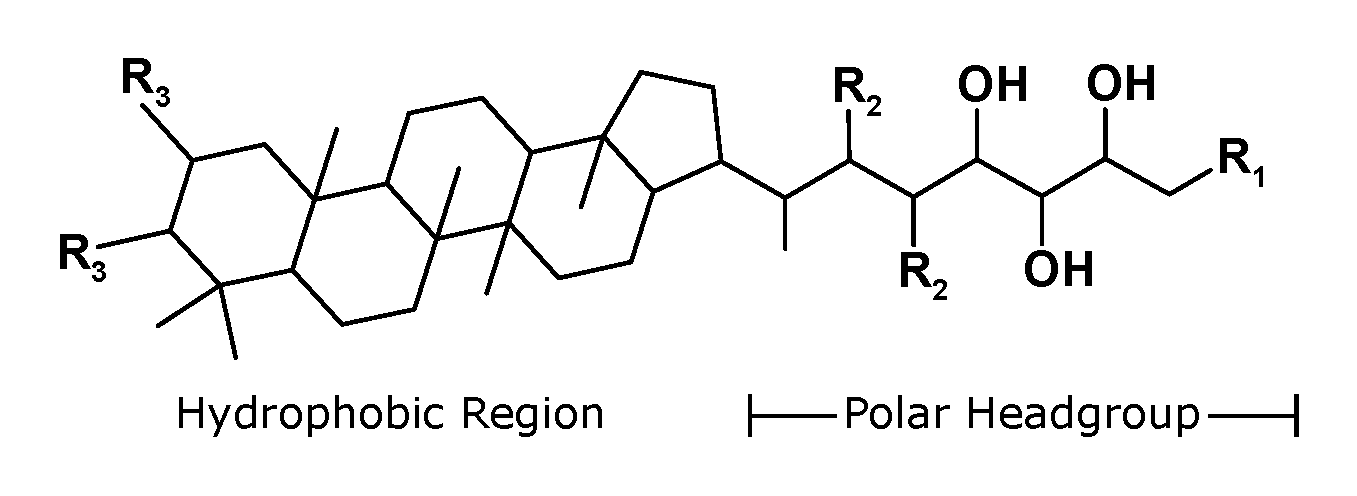
\includegraphics[width=1\linewidth]{figs_ch3/BHP_structure_general.pdf}
\caption[Generalized bacteriohopanepolyol chemical structure]{Generalized bacteriohopanepolyol (BHP) chemical structure. For BHPs without composite groups, R\textsubscript{1} represents a hydroxyl (OH), amine (NH\textsubscript{2}), or amminium (NH\textsubscript{3}\textsuperscript{+}) group. R\textsubscript{2} stands for H or OH. The BHP is considered pentafunctional if one R\textsubscript{2} is OH, or hexafunctional if both are OH. R\textsubscript{3} stands for H or CH\textsubscript{3}. Carbon positions 2, 3, and 35 are indicated.}
\label{fig:BHP_structure}
\end{figure}
\doublespace
\clearpage
}

The class of lipid chosen for this study was bacteriohopanepolyol (BHP), represented in Figure \ref{fig:BHP_structure}. BHPs are `C$_{35}$ hopanoids' (hopanoids containing 35 carbons) produced by a variety of bacteria. Hopanoids, with their specialized 5-ringed hydrophobic region, have been found to thicken and condense bacterial membranes and in a manner analogous to sterols in Eukaryotic organisms, demonstrated first by \cite{poralla1980glycolipid}. An experiment by \cite{poralla1984effect} showed that hopanoid abundance in \textit{Bacillus acidocaldarius} was strongly correlated with temperature, suggesting that hopanoids may play a role in membrane thermotolerance. \cite{welander2009hopanoids} observed defects in mutant cultures of \textit{Rhodopseudomonas palustris} strain TIE-1 lacking BHPs when grown under acidic or alkaline conditions, suggesting that these lipids may impart pH resistance. A study with mutant \textit{Burkholderia cenocepacia} also showed defects in the organism at low pH when unable to produce hopanoids, as well as poor swimming motility and decreased resistance to antibiotics and detergents \citep{schmerk2011hopanoid}. A study with cultures of ethanol-producing \textit{Zymomonas mobilis} concluded that hopanoid-fatty acid interaction conferred resistance to high ethanol concentrations \citep{bringer1985influence}. Examination of nitrogen-fixing vesicles in Frankia strains showed that the majority of lipids belonged to two BHP structures that are likely responsible for oxygen impermeability in these membranes \citep{berry1993hopanoid}. A study with \textit{Streptomyces coelicolor} found that hopanoid expression may help prevent escape of cytoplasmic water during aerial growth by condensing membranes \citep{poralla2000hopanoids}. Hopanoids are produced from the cyclization of squalene into diploptene by the enzyme squalene-hopene cyclase, SHC. Diploptene can be further modified by a series of Hpn enzymes to gain a polyfunctionalized aliphatic side-chain \citep{belin2018hopanoid, welander2012identification}, referred to in this work as a polar headgroup. BHPs are thought to orient in the membrane with the hydrophobic region facing inward and the polar headgroup facing outward, a notion supported by molecular dynamics simulations of bacteriohopanetetrol in a lipid bilayer \citep{poger2013relative}.

The hydrophobic region of BHPs tend to show little structural variation in living organisms. In most reports, a methylation may appear at either the C2 or C3 carbon position, or not at all. These methylations tend to be preserved in hopanoid structures in the geologic record, and for this reason there has been much study and discussion about their usefulness as biomarkers \citep[see review by][]{newman2016cellular}.

BHP headgroups exhibit a wide variety of structures. The C35 terminus of the headgroup can be decorated with a hydroxyl group or an amine. The number of headgroup hydroxylations can vary, resulting in 4, 5, or 6 total functional groups. Other organic molecules called `composite groups', such as aminosugars cyclitol and glucosamine, have been shown to link to the headgroups of some BHPs. Intriguingly, the specific functions served by BHP headgroup structures are still generally undiscovered (refs in Belin). We wanted to use this to our advantage; by treating each BHP heagroup as functionally equivalent, we wanted to know how well thermodynamic equilibrium could predict their distributions with respect to temperature and chemical composition of the surroundings.

In this study, we quantified structures of BHPs in thermophilic microbial communities sampled along the thermal and redox gradients of four YNP hot springs, Bison Pool (BP), Mound Spring (MS), Empress Pool (EP), and Octopus Spring (OS). To simplify subsequent thermodynamic calculations, we separated quantities of BHP headgroups into groups by degree of functionality (tetra-, penta-, and hexafunctional) and by aminopolyol and polyol. BHP composite groups were not considered. We then estimated the aqueous thermodynamic properties of the six resulting BHP headgroups; tetrol, pentol, hexol, aminotriol, aminotetrol, and aminopentol, as and the properties of the ionized forms of the aminopolyols, including amminiumtriol, amminiumtetrol, and amminiumpentol. Estimations of BHP headgroup aqueous thermodynamic properties were performed independently of observations of BHPs in hot spring samples and were based purely on thermodynamic measurements of organic molecules reported in the literature. Estimated BHP headgroup properties were then used in conjunction with measurements of hot spring temperature and chemical composition to predict equilibrium speciation of aqueous BHP headgroups along an Eh gradient, following the same principles one would use to predict aqueous carbonate speciation along a pH gradient. Relative abundance of BHP headgroups were then compared to these independent thermodynamic predictions of aqueous BHP headgroup speciation. Much like using measured abundances of carbonate species to predict pH, measured abundances of tetrafunctional and pentafunctional BHP headgroups were used to predict Eh in each sample. These BHP\textsubscript{BHP, head} values were compared to values of Eh previously reported for this sample set (Chapter \ref{ch2}) and were found to have a strong positive linear correlation, especially those calculated from the O\textsubscript{2}/H\textsubscript{2}O redox couple.

Eh\textsubscript{BHP, head} was predicted based only on the ratio of summed pentafunctional to tetrafunctional BHP headgroups. This was mostly due of the dominance of these headgroups among samples, but partly because thermodynamic predictions appeared to significantly overestimate the abundance of trace hexafunctional BHPs. Conversely, observed abundances of aminopolyols was underestimated by thermodynamic predictions by about 1-2 orders of magnitude. This opens the door to future work evaluating the sources of these discrepancies between predicted and observed BHP abundances; whether they stem from analytical uncertainty, underlying thermodynamic assumptions, or biological membrane functional requirements necessitating a higher energy cost.




\section{Methods}

\subsection{Water chemistry and metering}
Methods used to meter, collect, and analyze water samples are described in Chapter \ref{ch1} and \ref{ch2}. Briefly, temperature was metered with a YSI 30 conductivity meter and pH with a model 3300i or 3110 WTW pH meter with WTW probe. A Hach model 2400 or 2800 portable spectrophotometer and Hach reagents/protocols were used to measure concentrations of dissolved oxygen and sulfide in unfiltered water samples in the field. Samples for laboratory analysis were filtered down to 0.2 microns with Supor (Pall Corporation) filters and collected in 30 mL HDPE Nalgene bottles for ion chromatography and acid-washed amber glass vials with black butyl rubber septa for analysis of dissolved inorganic carbon (DIC). Concentrations of major cations and anions were obtained on Dionex DX-600 systems, while concentrations of DIC were measured on an OI Wet Oxidation TOC analyzer coupled to a Thermo Delta Plus Advantage mass spectrometer.

\subsection{Analysis of BHPs} Total lipid extracts (TLEs) from hot spring sediments and biofilms were obtained for this sample set as described in Chapter \ref{ch1}. Briefly, samples were collected with sterilized forceps and spatulas into sterile specimen containers and stored on dry ice the field before transferal into a -80$^{\circ}$C freezer. Samples were freeze-dried and homogenized with mortar and pestle prior to extraction with a modified version of the Bligh and Dyer method \citep{white1998signature}.

Aliquots of TLE set aside for BHP analysis were prepared for HPLC-MS as described in \cite{talbot2003atmospheric}. Briefly, BHPs were converted into their acetate derivative by heating aliquots of TLE in 1:1 v/v acetic anhydride and pyridine at 50$^{\circ}$ for 1 hour, leaving at room temperature overnight, drying under N$_2$, and then redissolving in methanol. Resulting TLEs were then injected Agilent 1200 Series HPLC equipped with a binary pump linked to an Agilent Q-TOF 6520 MS with a Poroshell 120 EC-C18 column and atmospheric pressure chemical ionization (APCI) source operated in positive ion mode. The column was first eluted isocratically with 100\% solvent A (95:5 MeOH:water) for 2 min, followed by a linear gradient to 20\% solvent B (isopropanol) for 18 minutes, then held isocratically for 10 min. The linear gradient continued to 30\% B over 10 min, held for 5 min, brought up to 80\% B over 1 min, then maintained for 14 min. The column was then eluted with 100\% A for 5 minutes. The flow rate throughout analysis was 0.19 mL min$^{-1}$.

BHPs were identified based on the exact masses of their protonated molecular ions at the MS level, their relative retention times, and by referencing MS/MS fragmentation patterns to published spectra \citep{talbot2005bacteriohopanepolyols, talbot2007rapid, talbot2007structural, talbot2003atmospheric, talbot2003characteristic, talbot2008cyanobacterial}. Diagnostic fragments m/z 191.18 and 205.20 indicating hopanoid C-ring cleavage were used to identify nonmethylated and methylated hopanoids, respectively. Tetra-, penta-, or hexafunctional BHPs were identified by fragments corresponding to the monoisotopic mass of acetylated polyol BHPs after loss of an acetyl or composite group fragment, namely m/z 655.49, 713.50, or 771.50 for polyol BHPs without a 2- or 3-methylation, and m/z 669.51, 727.51, or 785.52 for polyol BHPs with a 2- or 3-methylation. Aminopolyols were identified based on the m/z of the parent ion plus an proton adduct ([M + H]\textsuperscript{+}), and fragments at the MS/MS level indicating acetyl group loss. Aminopolyols with composite groups were not observed. Varying abundances of adenosylhopane and ribosylhopane were observed across samples, but were not included in this study because their headgroup functionality is not readily comparable to other BHPs, and because they might serve mainly as intermediates in BHP biosynthesis \citep{bradley2010adenosylhopane, liu2014ribosylhopane}. Anhydrobacteriohopanepolyols were observed but were not counted, as they are thought to be BHP degradation products \citep{talbot2005bacteriohopanepolyols, schaeffer2008acid}. Relative BHP within-sample abundances were obtained semi-quantitatively by comparing ratios of integrated peak areas of parent ions.



\subsection{Estimation of standard state thermodynamic properties of BHP polar headgroups.}
The workflow used to estimate standard state partial molal thermodynamic properties of aqueous BHP headgroups is shown schematically in Figure \ref{fig:BHP_thermoest_paper}. Estimations of tetra-, penta-, and hexafunctional BHP headgroups began with the properties of 1,2,3,4-butanetetrol, 1,2,3,4,5-pentanepentol, and 1,2,3,4,5,6-hexanehexol, respectively (structure A). The properties of these three sugar alcohols were be estimated by gathering available properties reported for aqueous sugar alcohol diastereomers (compiled in Table \ref{tab:sug_alc} along with their literature sources) and then regressing available $\Delta_{f}G^{\circ}_{aq}$, $\Delta_{f}H^{\circ}_{aq}$, $Cp^{\circ}_{aq}$, $V^{\circ}_{aq}$, and $\Delta_{h}G^{\circ}_{aq}$ as a function of carbon length. These regressions, which are shown in Figure \ref{fig:polyol_prop_regress}, were then used to solve for the properties of four, five, and six carbon-long isomer-agnostic sugar alcohols (given in Table \ref{tab:sa_regress}) used as structure A in the BHP headgroup estimation workflow.


\afterpage{
\singlespace
\begin{figure}[h]
\centering
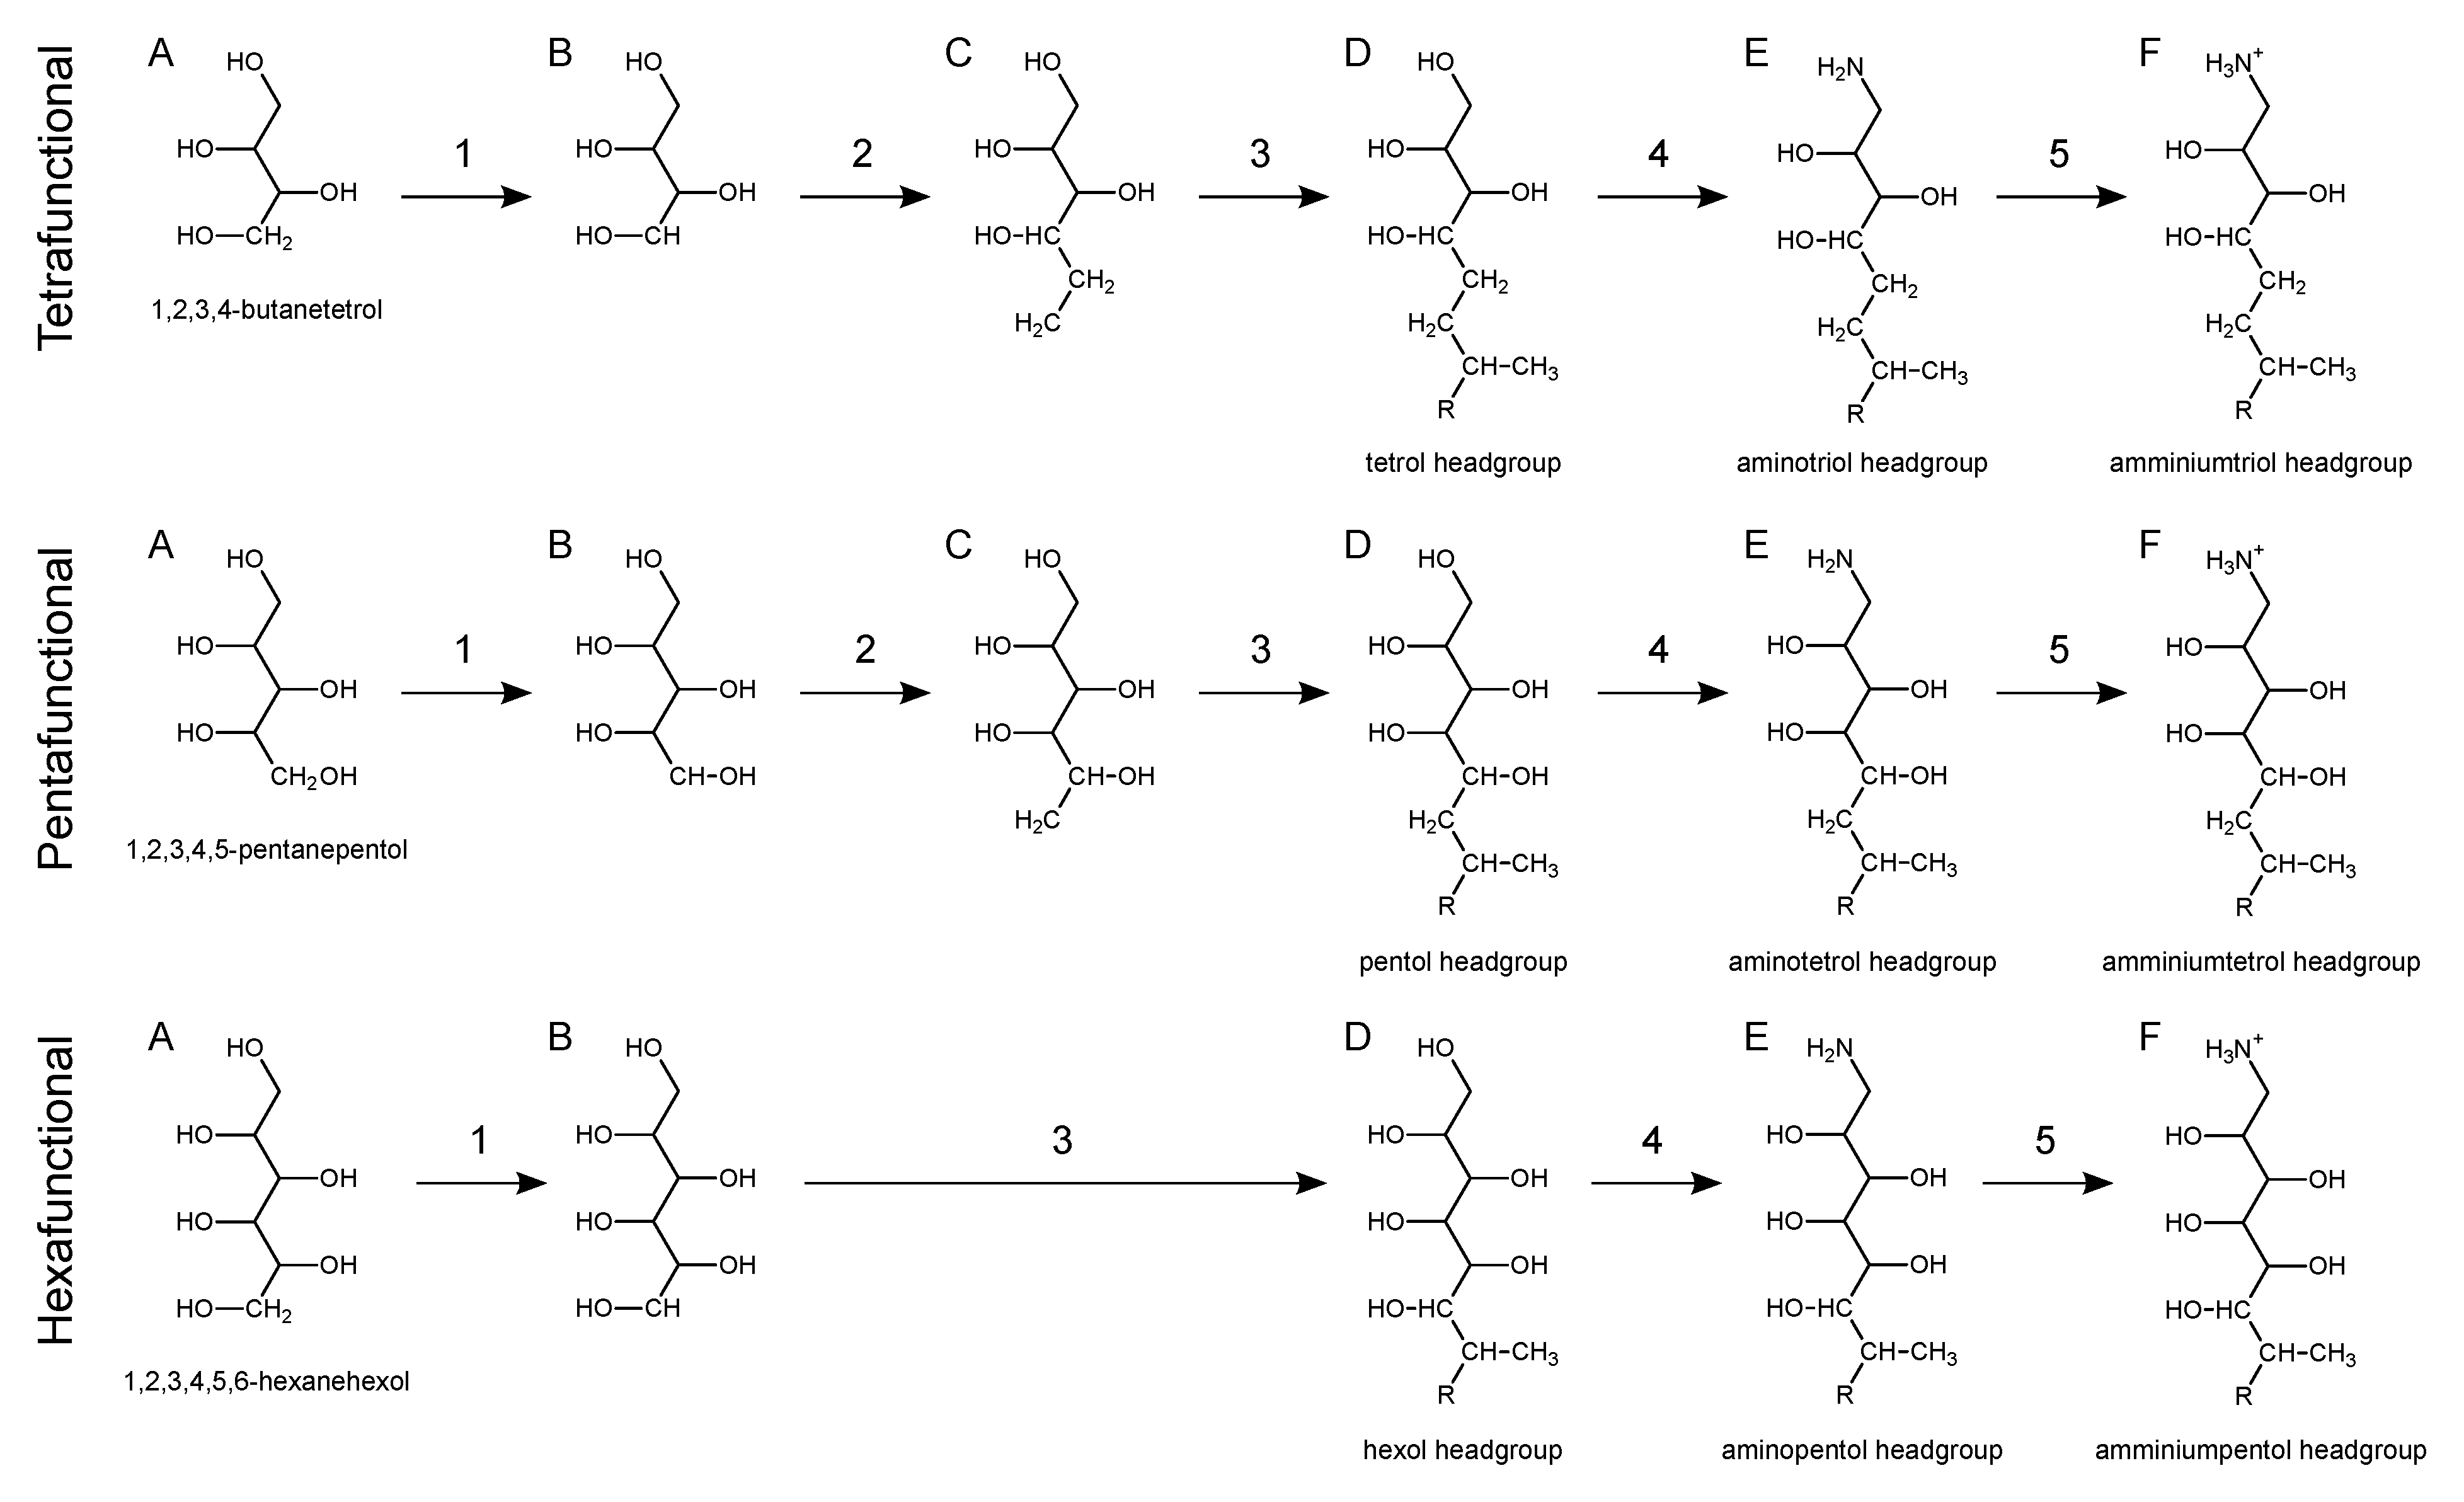
\includegraphics[width=1\linewidth]{figs_ch3/BHP_thermoest_paper.pdf}
\caption[Workflow used in the estimation of partial molal standard state thermodynamic properties of aqueous BHP headgroups]{Workflow used in the estimation of partial molal standard state thermodynamic properties of aqueous BHP headgroups. Structures and steps are described in the methods. R stands for the rest of the BHP structure, though its thermodynamic properties are not considered by this study.}
\label{fig:BHP_thermoest_paper}
\end{figure}
\doublespace
\clearpage
}


\afterpage{
% \newgeometry{margin=1.5cm} % modify this if you need even more space
% \centering
\begin{landscape}
\singlespace

\begin{table}
\centering
\begin{adjustbox}{width=600pt,keepaspectratio}
\begin{threeparttable}
  \caption{Partial molal thermodynamic data for sugar alcohols used in the estimation of BHP polar headgroup properties}

% Table generated by Excel2LaTeX from sheet 'Thermo sug alc'
\begin{tabular}{lrererererererererererererererer}
\toprule
      & \multicolumn{1}{l}{nC} & $\Delta_{f}G^{\circ}_{aq}$\rtr{SgAl_kjpermol} & $\Delta_{f}H^{\circ}_{aq}$\rtr{SgAl_kjpermol} & $Cp^{\circ}_{aq}$\rtr{SgAl_jpermolk} & $V^{\circ}_{aq}$\rtr{SgAl_cm3permol} & $\Delta_{h}G^{\circ}$\rtr{SgAl_kjpermol} & $\Delta_{h}H^{\circ}$\rtr{SgAl_kjpermol} & $\Delta_{sol}G^{\circ}$\rtr{SgAl_kjpermol} & $\Delta_{sol}H^{\circ}$\rtr{SgAl_kjpermol} & $\Delta_{sub}G^{\circ}$\rtr{SgAl_kjpermol} & $\Delta_{sub}H^{\circ}$\rtr{SgAl_kjpermol} & $\Delta_{sub}S^{\circ}$\rtr{SgAl_jpermolk} & $\Delta_{vap}H^{\circ}$\rtr{SgAl_kjpermol} & $\Delta_{f}G^{\circ}_{ig}$\rtr{SgAl_kjpermol} & $\Delta_{f}H^{\circ}_{ig}$\rtr{SgAl_kjpermol} & $S^{\circ}_{ig}$\rtr{SgAl_jpermolk} \\
\midrule
1,2-ethanediol & 2     & -333.3\rtr{GaqequalsGhplusGig} & -461.8\rtr{HaqequalsHhplusHig} & 193\rtr{lian1982polyol} & 54.60\rtr{dipaola1977polyol} & -32.9\rtr{plyasunov2006corresponding} & -72.9\rtr{hHsolHvapH} &       & -6.87\rtr{nichols1976thermochemistry} &       &       &       & 66.0\rtr{verevkin2004determination} & -300.4\rtr{GigHTdeltaS} & -388.9\rtr{verevkin20091} & 311.84\rtr{chao1986thermodynamic} \\
glycerol & 3     & -491.4\rtr{GaqequalsGhplusGig} & -675.4\rtr{bastos1988thermodynamic} & 240\rtr{lian1982polyol} & 70.91\rtr{dipaola1977polyol} & -51.1\rtr{plyasunov2006corresponding} &       &       &       &       &       &       &       & -440.3\rtr{verevkin2015thermodynamic} &       &  \\
erythritol & 4     &       &       & 310\rtr{lian1982polyol} & 87.1\rtr{dipaola1977polyol} & -51.9\rtr{GhGsolGsub} &       & -3.999\rtr{dehn1917comparative} &       & 47.9\rtr{GsubHsubTSsub} & 140\rtr{lopes2006determination} & 309\rtr{barone1990enthalpies} &       &       &       &  \\
threitol & 4     &       &       &       & 86.13\rtr{chavez1997hydrostatic} &       &       &       &       &       &       &       &       &       &       &  \\
xylitol & 5     & -791.87\rtr{da2013thermochemistry} & -1097.65\rtr{da2013thermochemistry} & 346\rtr{lian1982polyol} & 102.14\rtr{dipaola1977polyol} & -64.8\rtr{GhGsolGsub} &       & 4.0866\rtr{wang2013measurement} &       & 68.9\rtr{GsubHsubTSsub} & 161\rtr{barone1990enthalpies} & 309\rtr{barone1990enthalpies} &       &       &       &  \\
d-arabitol & 5     &       &       & 375\rtr{lian1982polyol} & 102.6\rtr{chavez1997hydrostatic} &       &       &       &       &       &       &       &       &       &       &  \\
l-arabitol & 5     &       &       & 373\rtr{lian1982polyol} & 102.6\rtr{chavez1997hydrostatic} &       &       &       &       &       &       &       &       &       &       &  \\
ribitol & 5     &       &       & 376\rtr{lian1982polyol} & 102.7\rtr{chavez1997hydrostatic} &       &       &       &       &       &       &       &       &       &       &  \\
iditol & 6     & -938.93\rtr{tewari1996thermodynamics} & -1309.94\rtr{tewari1996thermodynamics} &       &       &       &       &       &       &       &       &       &       &       &       &  \\
mannitol & 6     & -942.2\rtr{GaqequalsGhplusGig} &       & 452\rtr{lian1982polyol} & 119.71\rtr{dipaola1977polyol} & -97.5\rtr{GhGsolGsub} &       & -0.1162\rtr{dehn1917comparative} &       & 97.3\rtr{GsubHsubTSsub} & 202\rtr{barone1990enthalpies} & 351\rtr{barone1990enthalpies} &       &       &       &  \\
sorbitol & 6     & -944.49\rtr{tewari1996thermodynamics} & -1312.62\rtr{tewari1996thermodynamics} & 412\rtr{lian1982polyol} & 119.16\rtr{dipaola1977polyol} & -78.5\rtr{GhGfGig} &       &       &       &       &       &       &       & -866\rtr{yaws1997handbook} &       &  \\
galactitol & 6     &       &       &       & 118.6\rtr{chavez1997hydrostatic} &       &       &       &       &       &       &       &       &       &       &  \\
\bottomrule\end{tabular}%



  
  \begin{tablenotes}
    % The order of footnotes here will determine their letter in the table
    \tr{SgAl_kjpermol} kJ mol\textsuperscript{-1},
    \tr{SgAl_jpermolk} J mol\textsuperscript{-1} K\textsuperscript{-1},
    \tr{SgAl_cm3permol} cm\textsuperscript{3} mol\textsuperscript{-1},
    \tr{GaqequalsGhplusGig} calculated from $\Delta_{f}G^{\circ}_{aq} = \Delta_{h}G^{\circ} + \Delta_{f}G^{\circ}_{ig}$,
    \tr{HaqequalsHhplusHig} calculated from $\Delta_{f}H^{\circ}_{aq} = \Delta_{h}H^{\circ} + \Delta_{f}H^{\circ}_{ig}$,
    \tr{lian1982polyol} \cite{lian1982polyol},
    \tr{dipaola1977polyol} \cite{dipaola1977polyol},
    \tr{plyasunov2006corresponding} \cite{plyasunov2006corresponding},
    \tr{hHsolHvapH} calculated from $\Delta_{h}H^{\circ} = \Delta_{sol}H^{\circ} - \Delta_{vap}H^{\circ}$,
    \tr{nichols1976thermochemistry} \cite{nichols1976thermochemistry},
    \tr{verevkin2004determination} \cite{verevkin2004determination},
    \tr{GigHTdeltaS} calculated using $\Delta_{f}G^{\circ}_{ig}$ and $\Delta_{f}H^{\circ}_{ig}$ given in the table along with $S^{\circ}$ of the elements referenced from \cite{cox1989codata} and the relation $\Delta_{f}G^{\circ}_{ig} = \Delta_{f}H^{\circ}_{ig} - T\Delta(S_{ig}^{\circ}-\sum S_{elements}^{\circ}$),
    \tr{verevkin20091} \cite{verevkin20091},
    \tr{chao1986thermodynamic} \cite{chao1986thermodynamic},
    \tr{bastos1988thermodynamic} \cite{bastos1988thermodynamic},
    \tr{verevkin2015thermodynamic} \cite{verevkin2015thermodynamic},
    \tr{GhGsolGsub} calculated from $\Delta_{h}G^{\circ} = \Delta_{sol}G^{\circ} - \Delta_{sub}G^{\circ}$,
    \tr{dehn1917comparative} calculated using the relation $\Delta_{sol}G^{\circ} = -RT\ln{K_{sp}}$, where $R$ is the gas constant, $T$ is temperature, and $K_{sp}$ is the solubility product equilibrium constant calculated from the number of grams of sugar alcohol soluble per 100 grams of water at room temperature reported by \cite{dehn1917comparative},
    \tr{GsubHsubTSsub} calculated using $\Delta_{f}G^{\circ}_{sub}$ and $\Delta_{f}H^{\circ}_{sub}$ given in the table and the relation $\Delta_{f}G^{\circ}_{sub} = \Delta_{f}H^{\circ}_{sub} - T\Delta_{sub}S^{\circ}$),
    \tr{lopes2006determination} \cite{lopes2006determination},
    \tr{barone1990enthalpies} \cite{barone1990enthalpies},
    \tr{chavez1997hydrostatic} \cite{chavez1997hydrostatic},
    \tr{da2013thermochemistry} \cite{da2013thermochemistry},
    \tr{wang2013measurement} \cite{wang2013measurement},
    \tr{tewari1996thermodynamics} \cite{tewari1996thermodynamics},
    \tr{GhGfGig} calculated using values for $\Delta_{f}G_{aq}^{\circ}$ and $\Delta_{f}G_{ig}^{\circ}$ in the table and the relation $\Delta_{h}G^{\circ} = \Delta_{f}G_{aq}^{\circ} - \Delta_{f}G_{ig}^{\circ}$,
    \tr{yaws1997handbook} \cite{yaws1997handbook}
        
  \end{tablenotes}
  
  \label{tab:sug_alc}
  \end{threeparttable}
  \end{adjustbox}
\end{table}

% to get nicer header midrules, replace \cmidrule{3-8} with
% \cmidrule(l{2pt}r{2pt}){3-6} \cmidrule(l{2pt}r{2pt}){7-8}
\doublespace
\end{landscape}
% \restoregeometry
\setcounter{tabcounter}{0} % reset custom table footnote counter
\clearpage
}


\afterpage{
\singlespace
\begin{figure}[h]
\centering
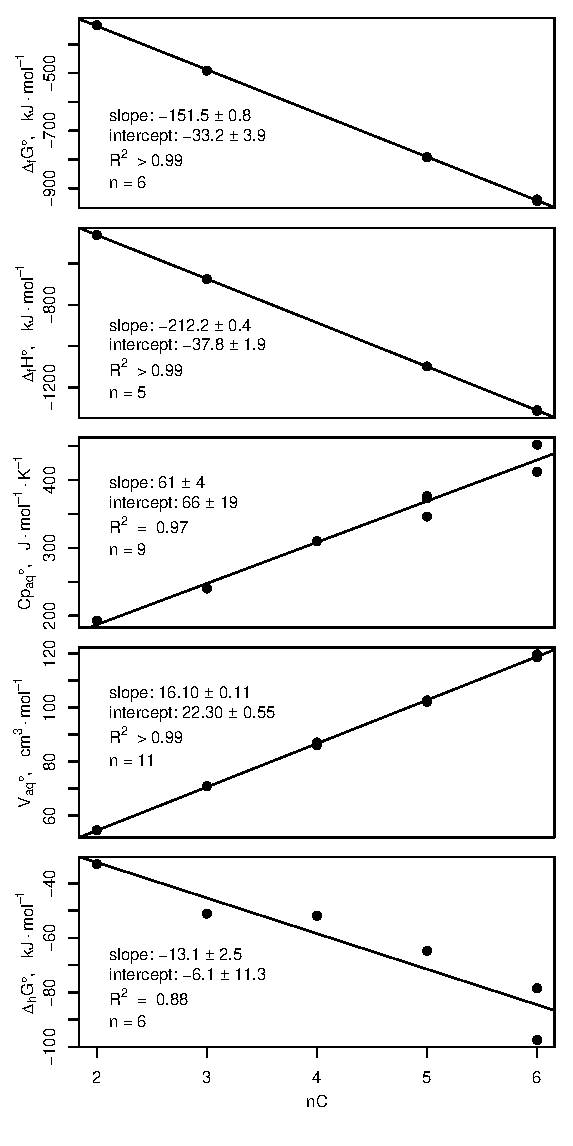
\includegraphics[width=0.5\linewidth]{figs_ch3/polyol_prop_regress.pdf}
\caption[Linear regression of experimentally-derived aqueous partial molal thermodynamic properties of sugar alcohols as a function of carbon length]{Linear regression of experimentally-derived aqueous partial molal thermodynamic properties of sugar alcohols as a function of carbon length (nC). Numbers of regressed datapoints for each plot are displayed equal to `n'. Literature sources for regressed data are given in Table \ref{tab:sug_alc}.}
\label{fig:polyol_prop_regress}
\end{figure}
\doublespace
\clearpage
}


\afterpage{
\singlespace
\begin{table}
\centering
\begin{threeparttable}
  \caption{Partial molal thermodynamic properties for non-stereoisomeric sugar alcohols estimated from the linear regression of sugar alcohol diasteromer properties given in Table \ref{tab:sug_alc} with carbon length, as shown in Figure \ref{fig:polyol_prop_regress}.}

% Table generated by Excel2LaTeX from sheet 'Thermo sug alc'
\begin{tabular}{lrererererer}
\toprule
      & \multicolumn{1}{l}{nC} & $\Delta_{f}G^{\circ}_{aq}$\rtr{sa_regress_kjpermol} & $\Delta_{f}H^{\circ}_{aq}$\rtr{sa_regress_kjpermol} & $Cp^{\circ}_{aq}$\rtr{sa_regress_jpermolk} & $V^{\circ}_{aq}$\rtr{sa_regress_cm3permol} & $\Delta_{h}G^{\circ}$\rtr{sa_regress_kjpermol} \\
\midrule
1,2,3,4-butanetetrol & 4     & -639.3 & -886.6 & 308   & 86.7  & -58.4 \\
1,2,3,4,5-pentanepentol & 5     & -790.9 & -1098.8 & 369   & 102.8 & -71.5 \\
1,2,3,4,5,6-hexanehexol & 6     & -942.4 & -1311.0 & 429   & 118.9 & -84.6 \\
\bottomrule
\end{tabular}%


  \begin{tablenotes}
    % The order of footnotes here will determine their letter in the table
    \tr{sa_regress_kjpermol} kJ mol\textsuperscript{-1},
    \tr{sa_regress_jpermolk} J mol\textsuperscript{-1} K\textsuperscript{-1},
    \tr{sa_regress_cm3permol} cm\textsuperscript{3} mol\textsuperscript{-1}
        
  \end{tablenotes}
  
  \label{tab:sa_regress}
  \end{threeparttable}
\end{table}
% to get nicer header midrules, replace \cmidrule{3-8} with
% \cmidrule(l{2pt}r{2pt}){3-6} \cmidrule(l{2pt}r{2pt}){7-8}
\setcounter{tabcounter}{0} % reset custom table footnote counter
\doublespace
\clearpage
}



\afterpage{
% \newgeometry{margin=1.5cm} % modify this if you need even more space
% \centering
\begin{landscape}
\singlespace

\begin{table}
\centering
\begin{adjustbox}{width=600pt,keepaspectratio}
\begin{threeparttable}
  \caption{Partial molal thermodynamic data for second order groups used in the estimation of BHP headgroup properties.}

% Table generated by Excel2LaTeX from sheet 'Thermo 2nd Order'
\begin{tabular}{llerererererererererererer}
\toprule
Group & Formula & $\Delta_{f}G^{\circ}_{aq}$\rtr{grpadd_kjpermol} & $\Delta_{f}H^{\circ}_{aq}$\rtr{grpadd_kjpermol} & $S^{\circ}_{aq}$\rtr{grpadd_jpermolk} & $Cp^{\circ}_{aq}$\rtr{grpadd_jpermolk} & $V^{\circ}_{aq}$\rtr{grpadd_cm3permol} & $\Delta_{h}G^{\circ}$\rtr{grpadd_kjpermol} & $\Delta_{h}H^{\circ}$\rtr{grpadd_kjpermol} & $\Delta_{h}S^{\circ}$\rtr{grpadd_jpermolk} & $\Delta_{h}Cp^{\circ}$\rtr{grpadd_jpermolk} & $\Delta_{f}H^{\circ}_{ig}$\rtr{grpadd_kjpermol} & $S^{\circ}_{ig}$\rtr{grpadd_jpermolk} & $Cp^{\circ}_{ig}$\rtr{grpadd_jpermolk} \\
\midrule
C-(H)(O)(C)\textsubscript{2} & CH    & 6.29\rtr{grpadd_GHS} & -27.98\rtr{grpadd_HaqHhHig} & -43.85\rtr{grpadd_SaqShSig} & 26\rtr{grpadd_CpaqCphCpig} & 7.48\rtr{plyasunov2004group} & -1.64\rtr{plyasunov2004group} & -1.88\rtr{plyasunov2004group} & -0.80\rtr{grpadd_GhHhSs} & 6\rtr{plyasunov2004group} & -26.10\rtr{domalski1993estimation} & -43.05\rtr{domalski1993estimation} & 19.96\rtr{domalski1993estimation} \\
C-(H)(C)\textsubscript{3} & CH    & 34.07\rtr{grpadd_GHS} & 1.17\rtr{grpadd_HaqHhHig} & -39.28\rtr{grpadd_SaqShSig} & 3\rtr{grpadd_CpaqCphCpig} & 5.96\rtr{plyasunov2004group} & -1.93\rtr{plyasunov2004group} & 2.34\rtr{plyasunov2004group} & 14.32\rtr{grpadd_GhHhSs} & -17\rtr{plyasunov2004group} & -1.17\rtr{domalski1993estimation} & -53.60\rtr{domalski1993estimation} & 20.08\rtr{domalski1993estimation} \\
C-(H)\textsubscript{2}(O)(C) & CH\textsubscript{2} & -4.41\rtr{grpadd_GHS} & -38.07\rtr{grpadd_HaqHhHig} & 23.51\rtr{grpadd_SaqShSig} & 88\rtr{grpadd_CpaqCphCpig} & 17.25\rtr{plyasunov2004group} & 0.77\rtr{plyasunov2004group} & -5.17\rtr{plyasunov2004group} & -19.92\rtr{grpadd_GhHhSs} & 68\rtr{plyasunov2004group} & -32.90\rtr{domalski1993estimation} & 43.43\rtr{domalski1993estimation} & 20.33\rtr{domalski1993estimation} \\
C-(H)\textsubscript{2}(C)\textsubscript{2} & CH\textsubscript{2} & 9.05\rtr{grpadd_GHS} & -24.15\rtr{grpadd_HaqHhHig} & 25.07\rtr{grpadd_SaqShSig} & 85\rtr{grpadd_CpaqCphCpig} & 15.61\rtr{plyasunov2004group} & 0.68\rtr{plyasunov2004group} & -3.52\rtr{plyasunov2004group} & -14.09\rtr{grpadd_GhHhSs} & 62\rtr{plyasunov2004group} & -20.63\rtr{domalski1993estimation} & 39.16\rtr{domalski1993estimation} & 22.89\rtr{domalski1993estimation} \\
C-(H)\textsubscript{3}(C) & CH\textsubscript{3} & -16.35\rtr{grpadd_GHS} & -50.45\rtr{grpadd_HaqHhHig} & 87.37\rtr{grpadd_SaqShSig} & 158\rtr{grpadd_CpaqCphCpig} & 25.56\rtr{plyasunov2004group} & 3.72\rtr{plyasunov2004group} & -8.19\rtr{plyasunov2004group} & -39.95\rtr{grpadd_GhHhSs} & 132\rtr{plyasunov2004group} & -42.26\rtr{domalski1993estimation} & 127.32\rtr{domalski1993estimation} & 25.73\rtr{domalski1993estimation} \\
\bottomrule
\end{tabular}%


  
  \begin{tablenotes}
    % The order of footnotes here will determine their letter in the table
    \tr{grpadd_kjpermol} kJ mol\textsuperscript{-1},
    \tr{grpadd_jpermolk} J mol\textsuperscript{-1} K\textsuperscript{-1},
    \tr{grpadd_cm3permol} cm\textsuperscript{3} mol\textsuperscript{-1},
    \tr{grpadd_GHS} calculated using $\Delta_{f}H^{\circ}_{aq}$ and $S^{\circ}_{aq}$ given in the table along with $S^{\circ}$ of the elements referenced from \cite{cox1989codata} and the relation $\Delta_{f}G^{\circ}_{aq} = \Delta_{f}H^{\circ}_{aq} - T\Delta(S_{aq}^{\circ}-\sum S_{elements}^{\circ}$),
    \tr{grpadd_HaqHhHig} calculated using $\Delta_{h}H^{\circ}$ and $\Delta_{f}H^{\circ}_{ig}$ given in the table and the relation $\Delta_{f}H^{\circ}_{aq} = \Delta_{h}H^{\circ} + \Delta_{f}H^{\circ}_{ig}$,
    \tr{grpadd_SaqShSig} calculated using $\Delta_{h}S^{\circ}$ and $S^{\circ}_{ig}$ given in the table and the relation $S^{\circ}_{aq} = \Delta_{h}S^{\circ} + S^{\circ}_{ig}$,
    \tr{grpadd_CpaqCphCpig} calculated using $\Delta_{h}Cp^{\circ}$ and $Cp^{\circ}_{ig}$ given in the table and the relation $Cp^{\circ}_{aq} = \Delta_{h}Cp^{\circ} + Cp^{\circ}_{ig}$,
    \tr{plyasunov2004group} \cite{plyasunov2004group},
    \tr{grpadd_GhHhSs} calculated using $\Delta_{h}G^{\circ}$ and $\Delta_{h}H^{\circ}$ given in the table and the relation $\Delta_{h}G^{\circ} = \Delta_{h}H^{\circ} - T\Delta_{h} S^{\circ}$,
    \tr{domalski1993estimation} \cite{domalski1993estimation}
        
  \end{tablenotes}
  
  \label{tab:grpadd}
  \end{threeparttable}
  \end{adjustbox}
\end{table}
\doublespace
\end{landscape}
% \restoregeometry
\setcounter{tabcounter}{0} % reset custom table footnote counter
\clearpage
}






\afterpage{
\singlespace
\begin{table}
\centering
\begin{threeparttable}
  \caption{Partial molal thermodynamic properties of aqueous chemical species used in the estimation of BHP aminopolyol headgroup properties.}

% Table generated by Excel2LaTeX from sheet 'Thermo misc'
\begin{tabular}{lererererer}
\toprule
      & $\Delta_{f}G^{\circ}_{aq}$\rtr{misc_kjpermol} & $\Delta_{f}H^{\circ}_{aq}$\rtr{misc_kjpermol} & $Cp^{\circ}_{aq}$\rtr{misc_jpermolk} & $V^{\circ}_{aq}$\rtr{misc_cm3permol} & $\Delta_{h}G^{\circ}$\rtr{misc_kjpermol} \\
\midrule
ethane & -16.29\rtr{orchyd} & -103.21\rtr{orchyd} &       &       &  \\
ethanol & -181.29\rtr{orchyd} & -287.2\rtr{orchyd} &       &       &  \\
methylamine &       &       &       &       & -19.1\rtr{ben1984solvation} \\
methylammonium &       &       &       &       & -315\rtr{pliego2000new} \\
ethylamine & 26.36\rtr{misc_shock1990calculation} & -99.705\rtr{misc_shock1990calculation} &       &       &  \\
ethanolamine & -138.64\rtr{Gethanolamineethylamineethanolethane} & -283.7\rtr{Hethanolamineethylamineethanolethane} & 176\rtr{cabani1981group} & 59.2\rtr{maham1994densities} & -18.9\rtr{pliego2000new} \\
ethanolammonium & -192.5\rtr{Gfethanolaminerxn} & -332.3\rtr{Hfethanolaminerxn} & 180.9\rtr{Cpethanolaminerxn} & 53.0\rtr{Vethanolaminerxn} & -305\rtr{pliego2000new} \\
\bottomrule
\end{tabular}%



  \begin{tablenotes}
    % The order of footnotes here will determine their letter in the table
    \tr{misc_kjpermol} kJ mol\textsuperscript{-1},
    \tr{misc_jpermolk} J mol\textsuperscript{-1} K\textsuperscript{-1},
    \tr{misc_cm3permol} cm\textsuperscript{3} mol\textsuperscript{-1},
    \tr{orchyd} recommended value from the ORganic Compounds HYDration properties (ORCHYD) database compiled by \cite{plyasunova2004database},
    \tr{ben1984solvation} \cite{ben1984solvation},
    \tr{pliego2000new} \cite{pliego2000new},
    \tr{misc_shock1990calculation} \cite{shock1990calculation},
    \tr{Gethanolamineethylamineethanolethane} estimated from $\Delta_{f}G^{\circ}_{aq, ethanolamine} = \Delta_{f}G^{\circ}_{aq, ethylamine} + (\Delta_{f}G^{\circ}_{aq, ethanol} - \Delta_{f}G^{\circ}_{aq, ethane})$,
    \tr{Hethanolamineethylamineethanolethane} estimated from $\Delta_{f}H^{\circ}_{aq, ethanolamine} = \Delta_{f}H^{\circ}_{aq, ethylamine} + (\Delta_{f}H^{\circ}_{aq, ethanol} - \Delta_{f}H^{\circ}_{aq, ethane})$,
    \tr{cabani1981group} \cite{cabani1981group},
    \tr{maham1994densities} \cite{maham1994densities},
    \tr{Gfethanolaminerxn} calculated from $\Delta_{f}G^{\circ}_{aq, ethanolammonium}$ and  $\Delta_{f}G^{\circ}_{aq, ethanolamine}$ in the table using the relation $\Delta_{f}G^{\circ}_{aq, ethanolammonium} = \Delta_{f}G^{\circ}_{aq, ethanolamine} - \Delta_{r}G^{\circ}_{d}$ where $\Delta_{r}G^{\circ}_{d}$ is the standard state Gibbs free energy of ethanolammonium dissociation taken as 53.90 kJ mol\textsuperscript{-1} from \cite{hamborg2009dissociation},
    \tr{Hfethanolaminerxn} calculated from $\Delta_{f}H^{\circ}_{aq, ethanolammonium}$ and  $\Delta_{f}H^{\circ}_{aq, ethanolamine}$ in the table using the relation $\Delta_{f}H^{\circ}_{aq, ethanolammonium} = \Delta_{f}H^{\circ}_{aq, ethanolamine} - \Delta_{r}H^{\circ}_{d}$ where $\Delta_{r}H^{\circ}_{d}$ is the standard state enthalpy change of ethanolammonium dissociation taken as 48.60 kJ mol\textsuperscript{-1} from \cite{hamborg2009dissociation},
    \tr{Cpethanolaminerxn} calculated from $Cp^{\circ}_{aq, ethanolammonium}$ and $Cp^{\circ}_{aq, ethanolamine}$ in the table using the relation $Cp^{\circ}_{aq, ethanolammonium} = Cp^{\circ}_{aq, ethanolamine} - \Delta_{r}Cp^{\circ}_{d}$ where $\Delta_{r}Cp^{\circ}_{d}$ is the standard state isobaric heat capacity change of ethanolammonium dissociation taken as -4.9 J mol\textsuperscript{-1} K\textsuperscript{-1} from \cite{bates1951acidic},
    \tr{Vethanolaminerxn} calculated from $V^{\circ}_{aq, ethanolammonium}$ and $V^{\circ}_{aq, ethanolamine}$ in the table using the relation $V^{\circ}_{aq, ethanolammonium} = V^{\circ}_{aq, ethanolamine} - \Delta_{r}V^{\circ}_{d}$ where $\Delta_{r}V^{\circ}_{d}$ is the standard state volume change of ethanolammonium dissociation taken as 6.2 cm$^3$ mol\textsuperscript{-1} from \cite{cabani1977volume}
        
  \end{tablenotes}
  
  \label{tab:misc_prop}
  \end{threeparttable}
\end{table}
% to get nicer header midrules, replace \cmidrule{3-8} with
% \cmidrule(l{2pt}r{2pt}){3-6} \cmidrule(l{2pt}r{2pt}){7-8}
\setcounter{tabcounter}{0} % reset custom table footnote counter
\doublespace
\clearpage
}



Steps one, two, and three of the workflow shown in Figure \ref{fig:BHP_thermoest_paper} involve the addition and subtraction of second order group contributions to thermodynamic properties given in Table \ref{tab:grpadd} to modify the properties of sugar alcohols (structure A) into those estimated for non-amino BHP headgroups (structure D). In step 1, the properties of structure B are obtained from structure A by subtracting the contribution from C-(H)\textsubscript{2}(O)(C), the properties of a CH\textsubscript{2} group bonded to one carbon and one oxygen, and adding the contribution from C-(H)(O)(C)\textsubscript{2}, the properties of a CH group bonded to two carbons and one oxygen. In step 2, the contribution of C-(H)\textsubscript{2}(C)\textsubscript{2}, a CH\textsubscript{2} group bonded to two carbons, is added to structure B a number of times such that structure C has six carbons. Step 2 is skipped for hexafunctional structure B, as it already has six carbons. In step 3, contributions from C-(H)(C)\textsubscript{3} and C-(H)\textsubscript{3}(C) are then added to structure C (or structure B for the hexafunctional workflow), resulting in estimated properties for six-carbon-long BHP tetrol, pentol, and hexol headgroups (structure D). In step 4, the properties of 1,2-ethanediol (given in Table \ref{tab:sug_alc}) are subtracted from structure D and those of ethanolamine (given in Table \ref{tab:misc_prop}) are added, resulting in the estimated properties of BHP aminotriol, aminotetrol, and aminopentol headgroups (structure E). In step 5, the properties of ionized aminopolyol BHP headgroups (structure F) are obtained by subtracting the properties of ethanolamine and adding those of ethanolamminium given in Table \ref{tab:misc_prop}.


\subsection{Estimation of revised Helgeson-Kirkham-Flowers (HKF) equation of state parameters for BHP polar headgroups}

Fitting parameters for the revised HKF equation of state were estimated for uncharged BHP polyol and aminopolyol headgroups using $\Delta_{f}G^{\circ}_{aq}$, $\Delta_{f}H^{\circ}_{aq}$, $Cp^{\circ}_{aq}$, $V^{\circ}_{aq}$, and $\Delta_{h}G^{\circ}_{aq}$ and the correlation strategies given in \cite{plyasunov2001correlation} for aqueous nonelectrolytes. Charged ammoniumpolyol BHP headgroups HKF parameters were estimated with a hybrid scheme, where the correlation strategy in \cite{sverjensky2014water} was used to estimate $a_{1}$ (for charged and uncharged aqueous species up to 60 kb), and the estimation methods in \cite{shock1990calculation} were used to obtain $\omega$ (from $S^{\circ}_{aq}$), $c_{1}$, $c_{2}$, $a_{2}$, and $a_{4}$. The parameter $a_{3}$ was solved from $\omega$ and the other $a$ parameters using the volume-dependent portion of the HKF equation, Equation A-1 in \cite{tanger1988calculation}.

\subsection{Calculating BHP headgroup metastable equilibrium abundance and headgroup-predicted Eh}

Methods used for calculating metastable equilibrium abundances for aqueous species as a function of Eh are described in Chapter \ref{ch2} for hypothetical site-average alkyl chains rather than for all observed chain structures, though in this study, the latter approach is taken. All nine polyol and aminopolyol BHP headgroup structures were allowed to speciate as a function of Eh. Observed ratios of tetrafunctional and pentafunctional BHPs in samples were compared to thermodynamically-predicted ratios along the calculated Eh gradient. Headgroup-predicted Eh was designated for a sample as the Eh where the relative ratio of tetrafunctional to pentafunctional BHP headgroups predicted by metastable equilibrium calculations matched the ratio observed in extracted BHPs (e.g. an observed ratio of 86:14 tetrafunctional to pentafunctional BHPs was observed in the lipid extract of sample BP2, and using the temperature and basis species concentrations of BP2, this ratio is predicted to be most stable at a an Eh of -0.164 volts; the headgroup-predicted Eh of BP2).



\afterpage{
% \newgeometry{margin=1.5cm} % modify this if you need even more space
% \centering
\begin{landscape}
\singlespace
% for evenly-spaced columns, use \begin{tabular}{llrerererererererererererer}

\begin{table}
\centering
\begin{adjustbox}{width=600pt,keepaspectratio}
\begin{threeparttable}
  \caption{Estimated thermodynamic standard state partial molal properties and Helgeson Kirkham Flowers equation of state parameters for aqueous BHP headgroups.}


% Table generated by Excel2LaTeX from sheet 'BHP chain properties'
\begin{tabular}{llrrrrrrrrrrrrr}
\toprule
BHP headgroup & formula & $\Delta_{f}G^{\circ}_{aq}$\rtr{kjpermol} & $\Delta_{f}H^{\circ}_{aq}$\rtr{kjpermol} & $S^{\circ}_{aq}$\rtr{jpermolk} & $Cp^{\circ}_{aq}$\rtr{jpermolk} & $V^{\circ}_{aq}$\rtr{cm3permol} & $a_{1}$\rtr{jpermolbar}$\times 10$ & $a_{2}$\rtr{jpermol}$\times 10^{-2}$ & $a_{3}$\rtr{jKpermolbar} & $a_{4}$\rtr{jKpermol}$\times 10^{-4}$ & $c_{1}$\rtr{jpermolk} & $c_{2}$\rtr{jKpermolbar}$\times 10^{-4}$ & $\omega$\rtr{jpermol}$\times 10^{-5}$ & $\Delta_{h}G^{\circ}$\rtr{kjpermol} \\
\midrule
tetrol & C\textsubscript{8}H\textsubscript{17}O\textsubscript{4} & -592.8 & -974.1 & 15.38 & 576   & 139.66 & 129   & 51.8  & 99.4  & -43.1 & 636   & -27.6 & 0.424 & -57.7 \\
pentol & C\textsubscript{8}H\textsubscript{17}O\textsubscript{5} & -753.4 & -1162.1 & 25.91 & 552   & 140.15 & 134   & 42.7  & 85.3  & -39.4 & 638   & -39.2 & 0.610 & -71.4 \\
hexol & C\textsubscript{8}H\textsubscript{17}O\textsubscript{6} & -914.0 & -1350.2 & 36.43 & 528   & 140.63 & 138   & 33.5  & 70.9  & -35.6 & 638   & -50.9 & 0.766 & -85.2 \\
aminotriol & C\textsubscript{8}H\textsubscript{18}NO\textsubscript{3} & -398.2 & -796.0 & 18.23 & 559   & 144.26 & 130   & 63.2  & 117   & -48.6 & 593   & -15.7 & 0.196 & -43.6 \\
aminotetrol & C\textsubscript{8}H\textsubscript{18}NO\textsubscript{4} & -558.8 & -984.1 & 28.76 & 535   & 144.75 & 134   & 53.8  & 103   & -44.6 & 595   & -27.3 & 0.420 & -57.4 \\
aminopentol & C\textsubscript{8}H\textsubscript{18}NO\textsubscript{5} & -719.4 & -1172.1 & 39.28 & 511   & 145.23 & 138   & 44.4  & 87.6  & -40.6 & 596   & -39.0 & 0.606 & -71.1 \\
amminiumtriol & C\textsubscript{8}H\textsubscript{19}NO\textsubscript{3}\textsuperscript{+} & -452.1 & -844.6 & 36.01 & 564   & 138.06 & 198   & -130  & -188  & 32.6  & 1110  & -259  & 1.84  & -330 \\
amminiumtetrol & C\textsubscript{8}H\textsubscript{19}NO\textsubscript{4}\textsuperscript{+} & -612.7 & -1033.0 & 46.53 & 540   & 138.55 & 202   & -139  & -204  & 36.8  & 1110  & -271  & 1.86  & -344 \\
amminiumpentol & C\textsubscript{8}H\textsubscript{19}NO\textsubscript{5}\textsuperscript{+} & -773.3 & -1220.7 & 57.06 & 516   & 139.03 & 206   & -149  & -220  & 41.0  & 1110  & -282  & 1.89  & -358 \\
\bottomrule
\end{tabular}%


  \begin{tablenotes}
    These values were generated as described in the methods.
    
    % The order of footnotes here will determine their letter in the table
    \tr{kjpermol} kJ mol\textsuperscript{-1},
    \tr{jpermolk} J mol\textsuperscript{-1} K\textsuperscript{-1},
    \tr{cm3permol} cm\textsuperscript{3} mol\textsuperscript{-1},
    \tr{jpermolbar} J mol\textsuperscript{-1} bar\textsuperscript{-1},
    \tr{jpermol} J mol\textsuperscript{-1},
    \tr{jKpermolbar} J K mol\textsuperscript{-1} bar\textsuperscript{-1},
    \tr{jKpermol} J K mol\textsuperscript{-1}


  \end{tablenotes}
  
  \label{tab:BHP_thermo_props}
  \end{threeparttable}
  \end{adjustbox}
\end{table}
\doublespace
\end{landscape}
% \restoregeometry
\setcounter{tabcounter}{0} % reset custom table footnote counter
\clearpage
}

\subsection{Calculating predicted fraction of aminopolyol BHP headgroups}

A separate calculation was performed to predict the abundance of aminopolyol BHP headgroups (aminotriol, aminotetrol, and aminopentol) relative to headgroups without amine functional groups (tetrol, pentol, hexol) in each sample. Calculations to predict relative abundance of BHP headgroups at the temperature and basis species concentrations were carried out as previously described. However, in reactions to form BHP headgroups from basis species, the concentration of electrons was set by headgroup-predicted Eh value for each sample rather than allowing it to be an independent variable. In this way, ratios of aminopolyols to polyols were predicted by thermodynamic calculations at Eh values that were themselves predicted from observed ratios of tetrafunctional and pentafunctional BHP headgroups.


\section{Results}

\subsection{Observed BHP headgroup functionality}

\afterpage{
\singlespace
\begin{figure}[h]
\centering
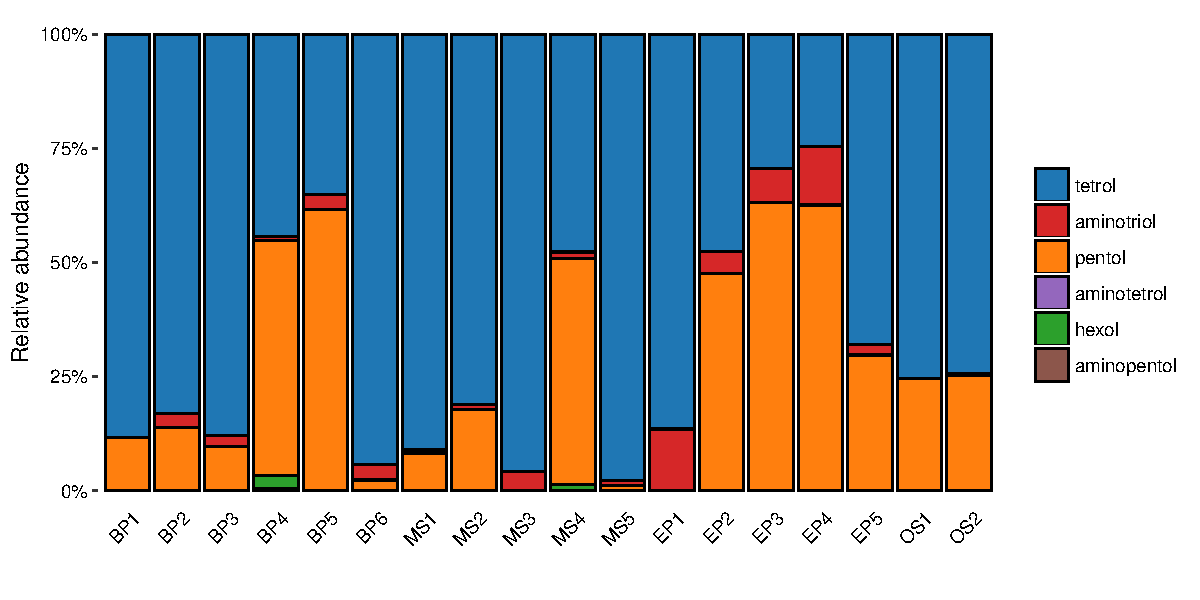
\includegraphics[width=1\linewidth]{figs_ch3/BHP_barchart.pdf}
\caption[Relative abundances of BHP polar headgroup functionality observed in Yellowstone hot spring sediments and biofilms]{Relative abundances of BHP polar headgroup functionality observed in Yellowstone hot spring sediments and biofilms.}
\label{fig:BHP_abund}
\end{figure}
\doublespace
\clearpage
}

Percent abundance of BHP headgroup functionality is shown for all hot spring samples in Figure \ref{fig:BHP_abund}. Tetrol (BHT with and without composite groups) was the dominant BHP headgroup in most samples, followed by pentols (BHpentol with and without composite groups). The ratio of pentol to tetrol saw a sharp increase in most samples representative of photosynthetic mats, such as BP4, BP5, and MS4. The mat sample of Octopus Spring, OS2, did not differ much from its upstream sample, OS1, however. Empress Pool, which did not have a visible cyanobacterial mat, still showed an increase in pentol to tetrol ratio within the temperature regime one would expect a photosynthetic mat in the other three springs. Interestingly, many samples that were most distal from their respective hot spring source, such as BP6, MS5, and EP5, saw a significant decrease in pentol to tetrol ratio. Samples BP6 and MS5 correspond to post-mat locations with microbial communities visually-distinct from those in the mat, and sample EP5, while relatively indistinguishable from samples immediately upstream from it, had a temperature about similar to MS5. BHPs with aminotriol headgroups were proportionally most abundant in samples belonging to Empress Pool, making up about 10\% of the total BHP headgroups observed at EP1 and EP4. Elsewhere, the abundance of aminotriol was rarely over 5\%. Aminotetrol was not observed in this sample set. Hexafunctional headgroups were observed in low abundance only in photosynthetic mat samples; with 2-5\% hexol in BP4 and MS4, and a trace amounts ($<$ 1\%) of aminopentol in BP4.

\subsection{Z\textsubscript{C} of BHP headgroups}

The weighted Z\textsubscript{C} of tetrafunctional, pentafunctional, and hexafunctional polyol and aminopolyol BHP headgroups (calculated for their non-composite form) are given in Table \ref{tab:BHP_redox_table}. Each step increase in the functionality of a BHP headgroup is accompanied by a change of +$0.3\overline{6}$ in Z\textsubscript{C}, and as such, samples with a greater ratio of higher-functionality BHP headgroups exhibited a higher weighted Z\textsubscript{C} . As shown in the top two panels of Figure \ref{fig:BHP_ZC_Eh_fourpanel}, weighted Z\textsubscript{C} did not have a strong linear correlation with temperature ($R^{2} = 0.20$) or Eh from the O\textsubscript{2}/H\textsubscript{2}O redox couple ($R^{2} = 0.06$), nor did it correlate with concentration of dissolved oxygen ($R^{2} = 0.16$, not shown). Unlike the clear, linear increase of alkyl chain Z\textsubscript{C} with decreasing temperature, the rise in BHP headgroup Z\textsubscript{C} downstream is punctuated by a sudden drop, indicating the onset of BHP headgroups with relatively reduced carbon in low temperature samples. Recall that BHP headgroups tetrol and pentol made up the majority of headgroups in this sample set, and that the pentol to tetrol ratio tended to be greatest in downstream mat samples spanning an approximate range of 40-74$^{\circ}$C, resulting in the relatively high Z\textsubscript{C} for BHP headgroups at these sites. The sudden decrease in pentol to tetrol ratio in the post-mat samples is responsible for the dip in Z\textsubscript{C} at the lowest-temperature sites.

\afterpage{
\singlespace
\begin{table}
\centering
% \begin{adjustbox}{width=\linewidth,keepaspectratio}
\begin{threeparttable}
  \caption{Select geochemical and physical data for samples, calculated and lipid-predicted redox potentials, and the average oxidation state of carbon in BHP headgroups.}


% Table generated by Excel2LaTeX from sheet 'TempEh_etc_noEh'
\begin{tabular}{ccccccc}
\toprule
      &       &       &       & Weighted Z\textsubscript{C} & \multicolumn{2}{c}{Lipid-predicted Eh, volts} \\
\cmidrule{6-7}Site  & Sample & T, $\degree$C & pH    & BHP headgroups & Eh\textsubscript{alkyl}\rtr{IPLtails} & Eh\textsubscript{BHP, head}\rtr{BHPheads} \\
\midrule
Bison & BP1   & 89.0  & 7.23  & -1.10 & -0.496 & -0.175 \\
Pool  & BP2   & 80.9  & 7.34  & -1.09 & -0.463 & -0.164 \\
      & BP3   & 73.3  & 7.27  & -1.09 & -0.435 & -0.153 \\
      & BP4   & 63.1  & 8.09  & -0.78 & -0.469 & -0.153 \\
      & BP5   & 40.5  & 8.25  & -0.42 & -0.397 & -0.110 \\
      & BP6   & 29.0  & 9.01  & -1.09 & -0.339 & -0.190 \\
      &       &       &       &       &       &  \\
Mound & MS1   & 91.0  & 8.81  & -1.10 & -0.606 & -0.299 \\
Spring & MS2   & 77.3  & 8.65  & -1.07 & -0.555 & -0.245 \\
      & MS3   & 64.8  & 9.08  & -1.13 & -0.553 & -0.292 \\
      & MS4   & 53.0  & 9.22  & -0.65 & -0.520 & -0.210 \\
      & MS5   & 35.1  & 9.53  & -1.12 & -0.441 & -0.251 \\
      &       &       &       &       &       &  \\
Empress & EP1   & 82.2  & 5.78  & -1.13 & -0.364 & -0.101 \\
Pool  & EP2   & 70.5  & 6.96  & -0.83 & -     & - \\
      & EP3   & 60.7  & 7.63  & -0.51 & -0.436 & -0.113 \\
      & EP4   & 51.6  & 7.99  & -0.60 & -0.426 & -0.120 \\
      & EP5   & 38.1  & 8.42  & -0.75 & -0.396 & -0.141 \\
      &       &       &       &       &       &  \\
Octopus & OS1   & 85.4  & 7.29  & -1.00 & -0.452 & -0.159 \\
Spring & OS2   & 59.8  & 8.27  & -0.83 & -0.482 & -0.176 \\
\bottomrule
\end{tabular}%


  \begin{tablenotes}
    Dashed entries represent samples where a particular Eh could not be calculated or estimated. See text.
    
    \tr{IPLtails} Eh predicted from alkyl chains of IPLs as reported in Chapter \ref{ch2},
    \tr{BHPheads} Eh predicted by BHP polar headgroups (this work)
        
  \end{tablenotes}
  
  \label{tab:BHP_redox_table}
  \end{threeparttable}
%   \end{adjustbox}
\end{table}
\doublespace
\setcounter{tabcounter}{0} % reset custom table footnote counter
\clearpage
}

\afterpage{
\singlespace
\begin{figure}[h]
\centering
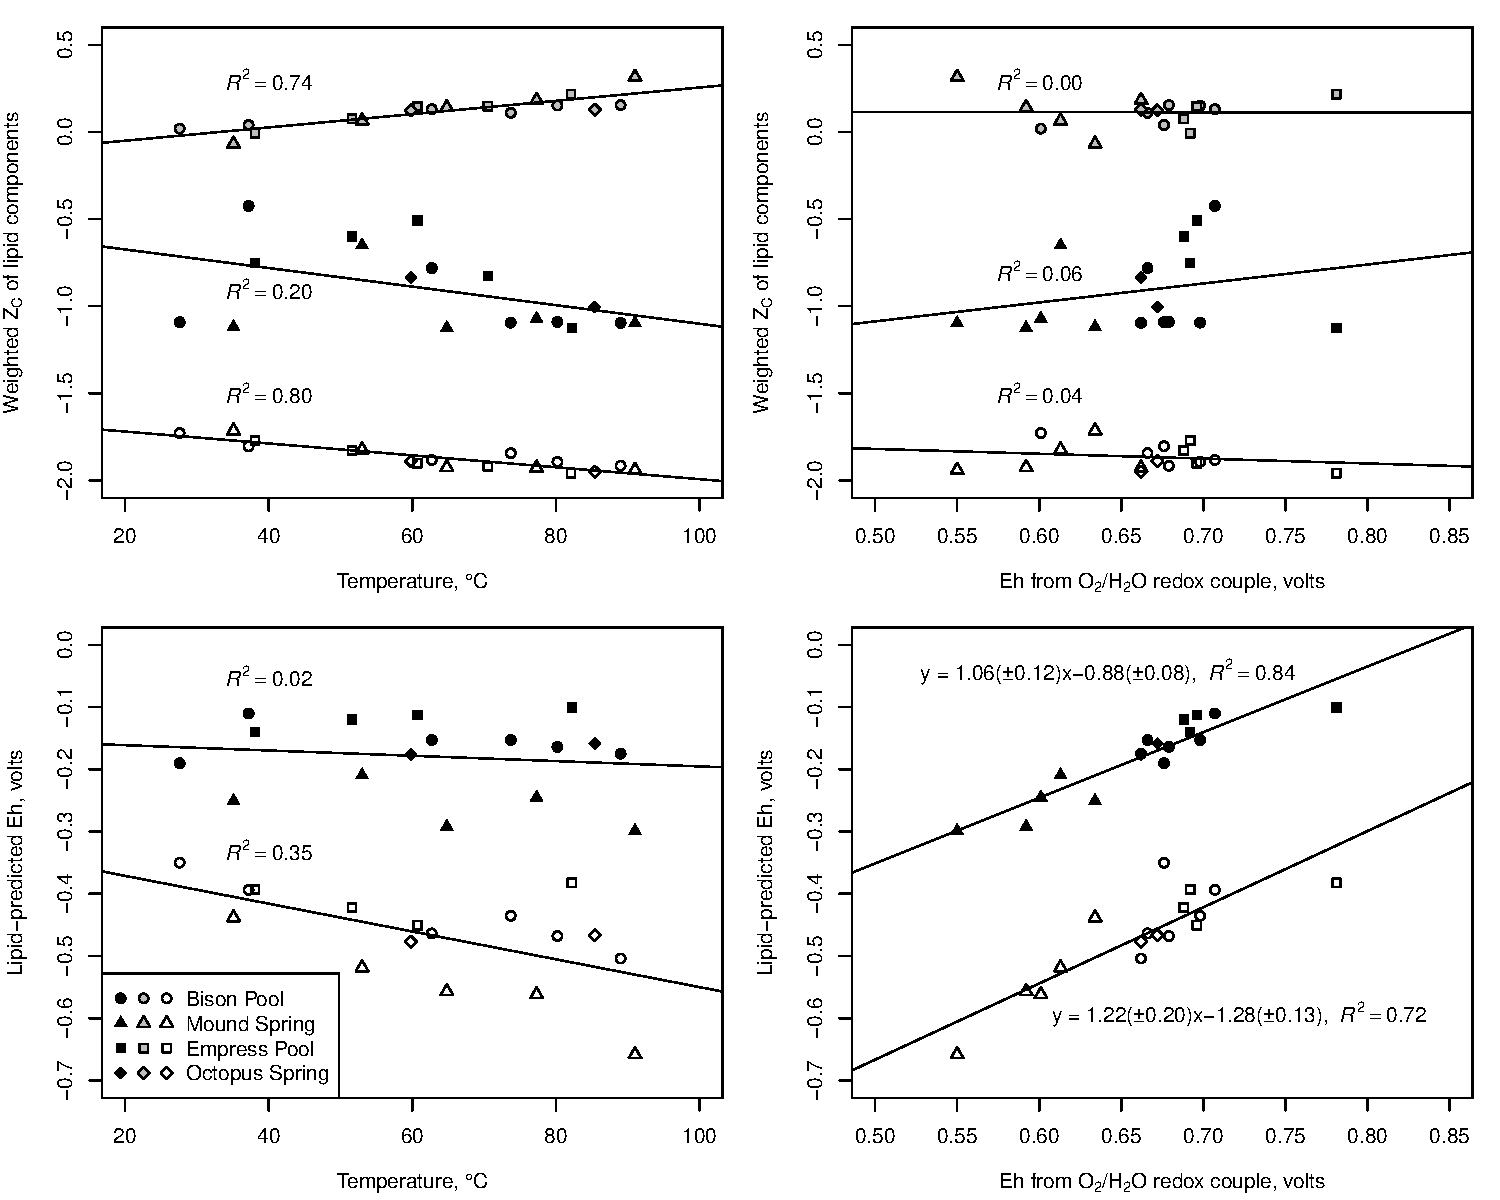
\includegraphics[width=1\linewidth]{figs_ch3/ZC_Eh_fourpanel.pdf}
\caption[Weighted Z\textsubscript{C} of thermophile lipid components and lipid-predicted Eh as a function of temperature and redox potential]{Weighted Z\textsubscript{C} of thermophile lipid components and lipid-predicted Eh as a function of temperature and redox potential. Black and gray symbols indicate headgroups of BHPs and IPLs, respectively. White/empty symbols indicate IPL alkyl chains in the upper plots or site-averaged IPL alkyl chains in the lower plots. Values for Z\textsubscript{C} of IPL components and alkyl chain-predicted Eh are taken from Chapters \ref{ch1} and \ref{ch2}, respectively. Standard errors of slopes and intercepts of linear fits are shown in parentheses and do not include propagated uncertainties from underlying thermodynamic estimations. Unweighted linear models were used to generate R\textsuperscript{2} values.}
\label{fig:BHP_ZC_Eh_fourpanel}
\end{figure}
\doublespace
\clearpage
}

Taken together, Z\textsubscript{C} as a predictive proxy for adaptation in BHP headgroup functionality temperature and chemical composition is not as easily interpretable as it appears to be for alkyl chains (Chapter \ref{ch1}). However, despite the linear correlation of alkyl chain Z\textsubscript{C} with temperature and co-varying log O\textsubscript{2} concentration, is interesting to note that the Z\textsubscript{C} of alkyl chains does \textit{not} appear correlated with Eh calculated from the O\textsubscript{2}/H\textsubscript{2}O redox couple (top right panel of Figure \ref{fig:BHP_ZC_Eh_fourpanel}). A more in-depth thermodynamic analyses was required to provide evidence that downstream alkyl chain distributions follows an energetically favorable trajectory with respect to both temperature chemical composition, including redox (Chapter \ref{ch2}, also see bottom right panel of Figure \ref{fig:BHP_ZC_Eh_fourpanel}). A similar approach was taken to predict whether observed distributions in BHP headgroup functionality are on an energetically favorable trajectory downstream in such a way that is not apparent with Z\textsubscript{C}.

\subsection{Thermodynamic predictions of Eh\textsubscript{BHP, head}}

\afterpage{
\singlespace
\begin{figure}[h]
\centering
    \begin{subfigure}[b]{\linewidth}
        \includegraphics[width=\linewidth]{figs_ch3/"Bison OF1_BHP_mosaic"}
        \label{fig:BP1_degform}
    \end{subfigure}
    \begin{subfigure}[b]{\linewidth}
        \includegraphics[width=\linewidth]{figs_ch3/"Bison OF2_BHP_mosaic"}
        \label{fig:BP2_degform}
    \end{subfigure}
\end{figure}

\newpage

\begin{figure}[h]\ContinuedFloat
    \begin{subfigure}[b]{\linewidth}
        \includegraphics[width=\linewidth]{figs_ch3/"Bison OF3_BHP_mosaic"}
        \label{fig:BP3_degform}
    \end{subfigure}\\[-4ex]
    \begin{subfigure}[b]{\linewidth}
    	\includegraphics[width=\linewidth]{figs_ch3/"Bison OF4_BHP_mosaic"}
        \label{fig:BP4_degform}
    \end{subfigure}
\end{figure}

\newpage

\begin{figure}[h]\ContinuedFloat
    \begin{subfigure}[b]{\linewidth}
        \includegraphics[width=\linewidth]{figs_ch3/"Bison OF5_BHP_mosaic"}
        \label{fig:BP5_degform}
    \end{subfigure}
    \begin{subfigure}[b]{\linewidth}
        \includegraphics[width=\linewidth]{figs_ch3/"Bison OF6_BHP_mosaic"}
        \label{fig:BP6_degform}
    \end{subfigure}\\[-4ex]

\caption[Predicted metastable equilibrium abundance of tetrafunctional and pentafunctional BHP headgroups in Bison Pool]{Predicted metastable equilibrium abundance of tetrafunctional (blue) and pentafunctional (orange) BHP headgroups in Bison Pool samples compared to observed ratios (blue to orange vertical arrow lengths) with corresponding BHP headgroup-predicted Eh indicated for each.}
\label{fig:BHP_degree_formation_bison}
\end{figure}
\doublespace
\clearpage
}

Tetrafunctional BHP headgroups are predicted to be stable in increasingly reduced conditions relative to pentafunctional headgroups, which are are stable in increasingly oxidized conditions, as shown in Figure \ref{fig:BHP_degree_formation_bison} for Bison Pool samples. At the temperature and basis species concentrations of sample BP1, metastable equilibrium calculations predict a fractional abundance of nearly 1 for tetrafunctional BHP headgroups an Eh of -0.2 volts and below, while pentafunctional headgroups are predicted to take over at an Eh above -0.08 volts. At approximately -1.45 volts, pentafunctional and tetrafunctional BHP headgroups are predicted to have the equal abundance, or a fractional abundance of 0.5 for each. Observed ratios of headgroup functionality in BHPs extracted from sample BP1 was about 12:88. The concentration of electrons in reactions to form BHP headgroups from basis species that would best predict a 12:88 penta- to tetrafunctionality ratio corresponds to an Eh\textsubscript{BHP, head} of -0.175 volts in sample BP1. In samples BP2 and BP3, similar ratios in functionality are observed (about 14:86 and 10:90, respectively), though increasingly oxidized conditions (-1.64 and -0.153 volts) are required predict these ratios due to a decrease in temperature and a shift in chemical composition. Sample BP4 represents the onset of the photosynthetic microbial mat and marks the first time in Bison Pool where pentafunctional headgroups become more abundant than tetrafunctional headgroups by a ratio of about 53:47. Intriguingly, metastable equilibrium predicts that at the temperature and basis species concentrations of BP4, the Eh\textsubscript{BHP, head} that best describes this headgroup functionality ratio is -0.153 volts, which is identical to that of BP3. An Eh\textsubscript{BHP, head} of -0.110, the most oxidized conditions predicted for Bison Pool yet, is needed to explain the pentafunctional to tetrafunctional headgroup ratio at BP5, which reached its peak of 62:38 for this spring. In the post-mat sample BP6, the abundance of pentafunctional headgroups had diminished substantially to a ratio of 2:98 predicted by an Eh\textsubscript{BHP, head} of -0.190 volts. Metastable equilibrium abundances of pentafunctional and tetrafunctional BHP headgroups as a function of Eh in Mound Spring, Empress Pool, and Octopus Spring samples are shown in Table \ref{fig:BHP_degree_formation}. Eh\textsubscript{BHP, head} values for all samples are given in Table \ref{tab:BHP_redox_table}.

Temperature does was not found to correlate with Eh\textsubscript{BHP, head} (R\textsuperscript{2} = 0.02), as shown in the bottom left panel of Figure \ref{fig:BHP_ZC_Eh_fourpanel}. When compared to the Eh predicted by site-averaged free alkyl chains of IPLs, Eh\textsubscript{alkyl}, which had a weak correlation, this may suggest that BHP structural adaptation may be less constrained by temperature than adaptations in alkyl chain structure. However, strong positive correlations were found between Eh\textsubscript{BHP, head} and sample Eh calculated from various redox couples reported in Table \ref{tab:eh_results} of Chapter \ref{ch2}; NO\textsubscript{2}\textsuperscript{-}/NO\textsubscript{3}\textsuperscript{-} (R\textsuperscript{2} = 0.74), NH\textsubscript{4}\textsuperscript{+}/NO\textsubscript{3}\textsuperscript{-} (R\textsuperscript{2} = 0.79), and HS\textsuperscript{-}/SO\textsubscript{4}\textsuperscript{2-} (R\textsuperscript{2} = 0.75). The strongest correlation was found between Eh\textsubscript{BHP, head} and Eh calculated from O\textsubscript{2}/H\textsubscript{2}O (R\textsuperscript{2} = 0.84, bottom right panel of Figure \ref{fig:BHP_ZC_Eh_fourpanel}). The slope of the trend was 1.06$\pm$0.12, suggesting a 1:1 relationship between Eh\textsubscript{O\textsubscript{2}/H\textsubscript{2}O} and Eh\textsubscript{BHP, head}. The regression of Eh\textsubscript{BHP, head} as a function of Eh\textsubscript{O\textsubscript{2}/H\textsubscript{2}O} runs approximately parallel to that of Eh\textsubscript{alkyl} but predicts an Eh that is about 0.40$\pm$0.14 volts more oxidized based on the difference in y-intercepts.

\subsection{Thermodynamic predictions of aminopolyol abundance}

\afterpage{
\singlespace
\begin{figure}[h]
\centering
    \begin{subfigure}[b]{0.45\linewidth}
        \includegraphics[width=1\linewidth]{figs_ch3/"scatterplot - predicted aminoBHPs vs observed"}
        \label{fig:amino_pred_obs}
    \end{subfigure}
    \begin{subfigure}[b]{0.45\linewidth}
        \includegraphics[width=\linewidth]{figs_ch3/"scatterplot - predicted aminoBHPs vs observed 04 RF"}
        \label{fig:amino_pred_obs_RF}
    \end{subfigure}
\caption[Predicted and observed fraction of aminopolyol BHP headgroups]{Predicted and observed fraction of aminopolyol BHP headgroups without response factor correction (left) and with a hypothetical response factor of 0.04x for aminopolyols relative to nonaminopolyols (right). Samples BP1 and OS2 are not plotted on this logarithmic scale because their observed fraction of aminopolyols was zero. ES2 is not plotted because a water sample was not collected, therefore a predicted abundance based on concentrations of basis species could not be performed for this sample.}
\label{fig:aminopolyol_predict}
\end{figure}
\doublespace
\clearpage
}

As shown in in the left panel of Figure \ref{fig:aminopolyol_predict}, the fraction of aminoBHPs in observed in lipid extracts is approximately 1-2 orders of magnitude greater than what is predicted by thermodynamic predictions of metastable equilibrium. This could be due to the sources of error in the way the thermodynamic properties of BHP headgroups were estimated, an unrepresentative choice of basis species, uncertainties in the underlying experimental data, \textit{etc}. It is possible that aminopolyol headgroup distributions in nature are responding to variables that are not captured in this thermodynamic model or its underlying energetic assumptions. If one assumes the reverse is true, the discrepancy between predicted and observed fractions could be explained potential differences in ionization efficiency between BHPs with aminopolyol and polyol headgroups during LC-MS analysis. Due to a lack of commercially-available standards, response factor correction could not be performed during the quantification of BHP structures. For the fraction of predicted aminopolyol headgroups to approach observation, BHP LC-MS integrated peak areas would need a response factor correction of about 0.04x, or 25x for non-aminopolyols (Figure \ref{fig:aminopolyol_predict}, right panel). This is not outside the realm of possibility; \cite{cooke2008bacterial} and \cite{van2012bacteriohopanepolyol} reported that  peak areas of BHPs with nitrogen were approximately 12/8 as intense as those without among a suite of five BHP standards. That roughly translates to a response correction of about 8/12x, or 0.7x, to nitrogen-bearing BHP peak areas to bring them into approximate consistency with BHPs without nitrogen. It should be noted that these response factors were obtained using a different set of instrumentation than that used in this study, so reported response factors may not represent peak area correction values relevant to this analysis. That said, general differences in response factors have been observed between nitrogenous and non-nitrogenous authentic lipid standards on the same LC-MS model used in this study; though these standards were non-BHP intact polar lipids. As described in Chapter \ref{ch1}, many of the response factor assignments to lipids in samples without a representative headgroup standard were guided by the presence or absence of nitrogen in their chemical structure, as peak area intensity of standards with nitrogen tended to be greater than those without. This is not proof that BHP peak areas would behave in this way, since relative peak area intensity of analytes could be greatly affected by the LC method and mass spectrometer ionization source (which are not the same between the analysis of IPLs in Chapter \ref{ch1} and BHPs in this study), though the principle that aminopolyol and polyol BHPs may have different response factors remains plausible.

%%% results notes:
% If time, do something with hexafunctional BHPs. E.g. "predicted fraction of hexafunctional" based on observed ratio of pent and tet. Including hexafunctional BHPs hardly (if at all) changes BHP-predicted Eh from pent and tet.

% If time, thermodynamic calculation results:
% (briefly) Regression results for sugar alcohols. Good correlation for most properties. Gibbs free energy of hydration's correlation not as good as others.

\section{Discussion}

The thermodynamic predictions of BHP headgroup favorability along an Eh gradient performed in this work were carried out in a similar fashion to the estimations performed on site-averaged alkyl chains in Chapter \ref{ch2}. However, rather than calculating thermodynamic properties of hypothetical site-average lipid structures, this study aimed at estimating the thermodynamic properties of observed aqueous BHP polar headgroup structures reported in the literature, and then using properties to calculate equilibrium abundances of BHP headgroups along an Eh gradient. The Eh value that predicted equilibrium-abundance BHP ratios that matched ratios observed in a sample lipid extract was denoted the `BHP headgroup-predicted Eh' (BHP\textsubscript{BHP, head}) for that sample. These values of BHP\textsubscript{BHP, head} were then compared to the Eh values calculated for samples from inorganic species reported in Chapter \ref{ch2} in to determine whether there was a strong positive correlation. Such a correlation would suggest that abundances of BHP headgroups are following an energetically favorable trajectory in the context of hot spring temperature and chemical composition. The contribution of the BHP hydrophobic region was not included in thermodynamic calculations because their structure is relatively conserved between BHPs and was not expected to effect predicted BHP headgroup distributions significantly.

The results in BHP\textsubscript{BHP, head} can perhaps be best discussed in context of a more familiar example; carbonate speciation with pH. As shown in Figure \ref{fig:carbonate_speciation}A, aqueous carbonate species chemically speciate at room temperature as a function of pH according to thermodynamic equilibrium. Carbon dioxide (CO\textsubscript{2}) is the dominant species below about pH 6.2, bicarbonate (HCO\textsubscript{3}\textsuperscript{-}) between 6.2 and 10.3, and carbonate (CO\textsubscript{3}\textsuperscript{2-}) above 10.3. Assuming that one did not know the pH of the system but could measure the concentration of carbonate species, the fractional abundance of carbonate could be used to solve for pH. For instance, a measured ratio of 75:25 CO\textsubscript{3}\textsuperscript{2-} to HCO\textsubscript{3}\textsuperscript{-} would indicate a pH of about 10.8 at room temperature, or a pH of about 10.6 at 90$^{\circ}$C (Figure \ref{fig:carbonate_speciation}B). Fractional abundance at 90$^{\circ}$C was calculated from equilibrium constants predicted by the revised Helgeson-Kirkham-Flowers (HKF) equation of state \citep{shock1992calculation} and thermodynamic data and parameters reported in \cite{shock1988calculation} and \cite{plyasunov2001correlation} for aqueous carbonate species.

\afterpage{
\singlespace
\begin{figure}[h]
\centering
    \begin{subfigure}[b]{1\linewidth}
        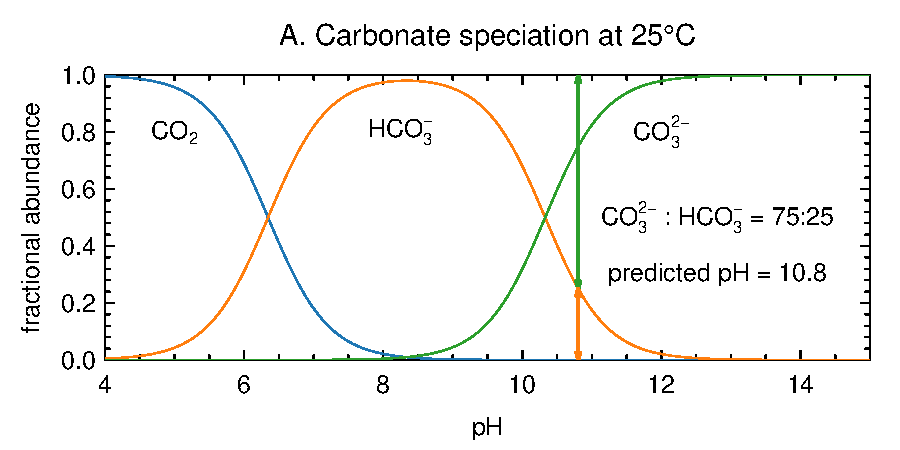
\includegraphics[width=1\linewidth]{figs_ch3/CarbonateExample25C}
        \label{fig:carbonate25}
    \end{subfigure}
    \begin{subfigure}[b]{1\linewidth}
        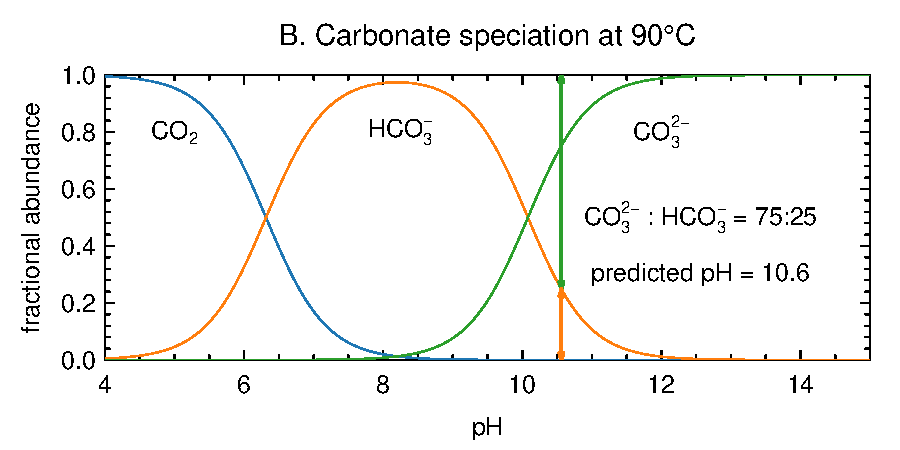
\includegraphics[width=1\linewidth]{figs_ch3/CarbonateExample90C}
        \label{fig:carbonate90}
    \end{subfigure}
\caption[Predicted fractional abundance of aqueous carbonate species as a function of pH]{Predicted fractional abundance of aqueous carbonate species as a function of pH at 25$^{\circ}$C (A) and 90$^{\circ}$C (B). Vertical arrows show the pH predicted by a ratio of 75:25 CO\textsubscript{3}\textsuperscript{-2} to HCO\textsubscript{3}\textsuperscript{-}.}
\label{fig:carbonate_speciation}
\end{figure}
\clearpage
\doublespace
}

Reaction kinetics are rapid in the carbonate system, so a shift in pH results in a near-immediate re-equilibration of carbonate species into the fractional abundance at the new pH. In a hypothetical system where microbial membrane lipids are allowed to interchange rapidly in response to the chemical and thermal context of the surroundings, similar observations might be expected with respect to the fractional abundance of BHP headgroups; an increase in ammonia concentration might favor an increase in the fractional abundance of nitrogen-bearing aminopolyols. Likewise, a shift from relatively reduced to oxidized redox potential might favor the fractional abundance of BHP headgroups with a greater number of oxidized functional groups. As with the carbonate system, BHP headgroup fractionation would then represent the most thermodynamically stable equilibrium abundances based on the temperature and chemical conditions of the surroundings. By measuring the fractional abundance of BHP headgroups, it would then be possible to solve for a single chemical unknown assuming all other relevant chemical variables are known, much like predicting pH from the fraction of aqueous carbonate species. Furthermore, if thermodynamic properties were available for aqueous BHP headgroups, the HKF equation could be used to solve for a chemical unknown at elevated temperatures, such as those found in hot springs.

Based on what is known about BHP biosynthetic pathways in bacteria, however, it is unlikely that a change in chemical composition would result in reconfiguration of BHP headgroups at a rate even remotely comparable to that of the carbonate system. The BHP formylhopane is thought to be a precursor molecule that can either be reduced to a tetrol headgroup, or aminated to an aminotriol headgroup by the aminotransferase HpnO \citep{welander2012identification}. Therefore, it is unlikely that there would be a direct reaction of a polyol heagroup with ammonia to form an aminopolyol headgroup, as was posited earlier. This does not preclude the possibility that thermodynamic equilibrium among BHP headgroups could be converged upon indirectly; increased ammonia concentration might drive the glutamate dehydrogenase-catalyzed reaction of $\alpha$-ketoglutarate to form glutamate \citep{lightfoot1988expression}, followed by the HpnO-catalyzed reaction of glutamate and formylhopane to $\alpha$-ketoglutarate and a BHP aminopolyol, conceivably leading to an increase in the fractional abundance of aminopolyol BHP headgroups.  However, experiments performed on \textit{Desulfovibrio bastinii} showed no obvious difference in aminopolyol headgroup fraction between cultures growing with and without ammonium \citep{blumenberg2012novel}, though it should be noted that the studied microorganism was capable of fixing its own nitrogen. It is still uncertain, then, whether bacteria metabolically shift fractional abundances of their BHP headgroups into configurations approaching thermodynamic equilibrium (at least in the case of ammonia and aminopolyols).

Whether or not bacteria shift their BHP headgroup distributions in such a way that approaches thermodynamic equilibrium within short, observable timescales, thermodynamically favorable assemblages of BHP headgroups may still be converged upon over the course of evolution. Life is not a system at equilibrium, so thermodynamic predictions of biolomecular compositions may only be expected to go so far. However, life must still obey the laws of thermodynamics, and must construct itself out of the nutrients and energy supplies available to it. Organisms that make the best use of their surroundings have a competitive edge, and are said to be `adapted'. It is conceivable that organisms would save cellular energy over the course of evolution by adapting functional biomolecules that are cost-effective in the temperature and chemical composition of their surroundings, or in other words, minimizing the Gibbs free energy of reactions to form biomolecules from available chemical species. These Gibbs free energies may never reach 0, but trends suggesting minimization could indicate an evolutionary approach toward equilibrium such that energy is saved while remaining competitive.

Equilibrium assumptions were used to evaluate observations of BHP headgroup distributions as a function of temperature and Eh. These thermodynamically-predicted Eh values had a strong positive correlation with Eh independently-calculated from measured concentrations of redox-sensitive inorganic species. These trends suggest that BHP headgroup compositions have adapted to remain functional while minimizing Gibbs free energy of formation from available chemical species. In sum, observed abundances of BHP headgroups in this work may represent energetically-driven distributions to provide functional membranes along natural thermal and chemical gradients.



% Possible discussion material
% First, revisit carbonate system from intro
% Revisit equilibrium assumptions. Essentially; life is not in equilibrium. However, it still has to make itself from nutrients and energy supplies available to it. Organisms that make the best use of their surroundings have a competitive edge, and are said to be 'adapted'. One way that an organism can make the best use of its surroundings is by substituting readily-available materials into its biomolecules. Even if the substituted biomolecule does not function as well, the energy saved could be diverted elsewhere in the organism to provide an overall net competitive advantage. This natural cost/benefit analysis may be the reason why we see changes in metagenome-encoded peptide sequences change in an energetically-favorable way along a temperature/redox gradient (Jeff), or why lime disease spirochete no longer requires iron, or why genomically encoded survival mechanisms offer alternative pathways for creating substituted molecules (iron and vanadium nitrogenases, nitrogen lipids in place of phospholipids). So how does an organism save biosynthetic energy in in over the course of evolutionary history? One strategy might be to make functional biomolecules out of what's available. Minimize the gibbs free energy of the reaction to form the biomolecule out of available materials. Potentially less ATP or NADH(P) or proton gradient or whatever is needed that way.

% final point: observed BHP composition may reflect adaptations that are energetically-driven. Minimization of gibbs free energy of reactions forming BHPs. Use equilibrium thermodynamic assumptions and observations of thermal and geochemical conditions to evaluate 'Eh', which is unknown (also, system does not have one Eh). Although there is no single Eh, there are Eh TRENDS. Does Eh predicted from headgroups correlate positively with Eh from inorganic species? If so, provides evidence that observed BHP distributions in microbial communities are approaching to equilibrium with respect to their biomolecular composition -> saving energy -> adaptation. May not be AT equilibrium, but doing best to approach it while remaining competitive.

% Future work - constraining aminopolyol and hexafunctional predictions. Do hexafuntional BHPs have a different function altogether? Too many hydroxyl groups to be functional in most membranes?

% Previous work showed that ZC of IPLs increased with temperature or DO and that changes in the nonpolar tailgroups were mainly responsible. The ZC of IPL headgroups, however, did not follow this trend. The question arises, is this trend purely a result of the semiquantitative nature of the analysis (response factors, etc.) that tailgroups are less susceptible to, or a reflection of a real trend? If the latter is true, does going against the ZC trend cost extra?

% Like IPL headgroups, the weighted ZC of BHP headgroups does not behave with temperature, O2, or Eh. Does this imply increased cost?
% Estimating the thermodynamic properties of BHP headgroups and then using actual ratios of pentafunctional to tetrafunctional headgroups to predict Eh (using methods independent of O2, Eh, etc.) results in a strong correlation with EQ3-calculated Eh from the O2/H2O redox couple (and other co-varying couples).
% Observed ratios of tetrafunctional and pentafunctional BHPs may represent the most thermodynamically stable assemblage for the set of environmental redox conditions.


% discussion point, was talked about in results a little: downstream increase of ZC was a good proxy for energetic favorability predicted by thermodynamic calculations involving IPL alkyl chains, though as shown in topright of four panel figure, zc of alkyl chains does not trend with Eh. It required a more in-depth thermodynamic assessment to show that increasing Eh calculated by O2/H2O correlated positively with energetic favorability of alkyl chains.

%%%%
